\documentclass{beamer}
    \usepackage{../inc/ssbeamer}

    \title{Boids}
    \subtitle{Grupo 01}

    \begin{document}

    \frame{\titlepage}

    \section{Fundamentos}
    \begin{frame}
        \frametitle{Boids: Reglas}
        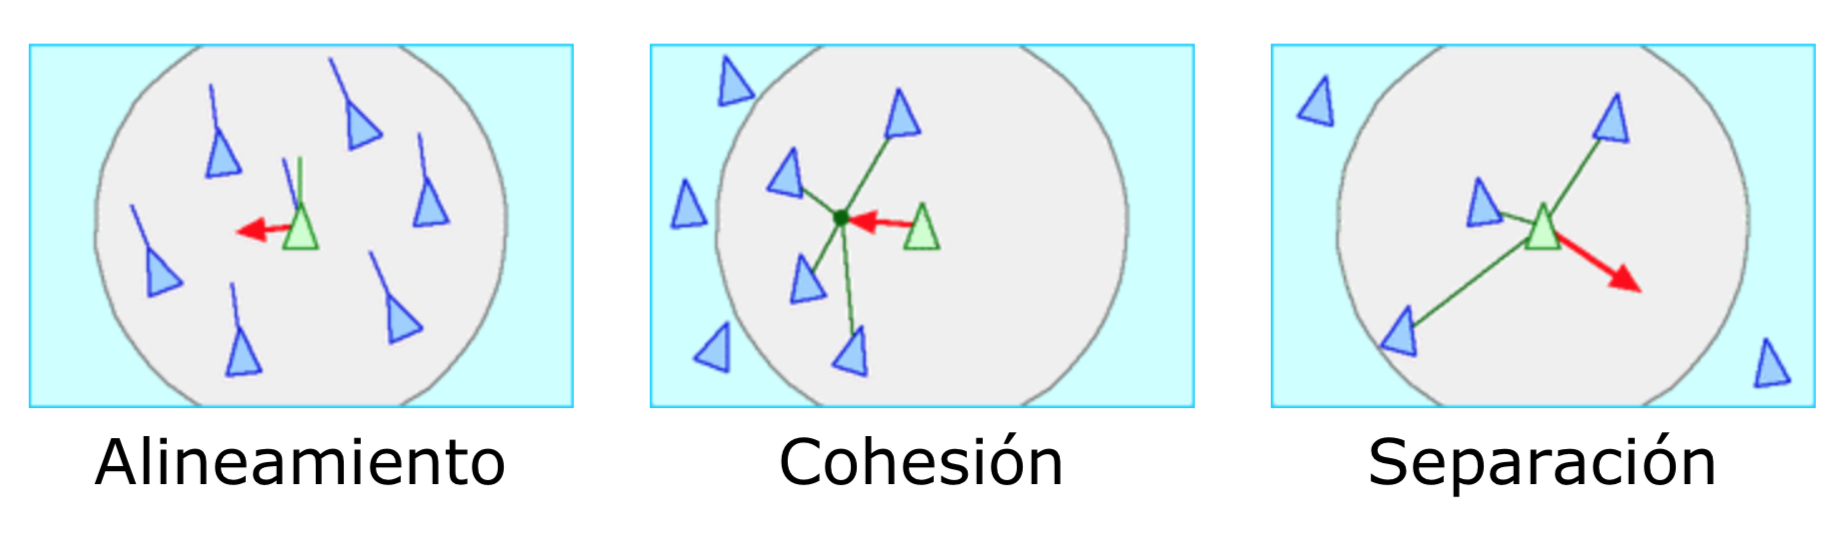
\includegraphics[width=\linewidth,height=\textheight,keepaspectratio]{{../imgs/rules_overview}.png}
    \end{frame}
    \begin{frame}
        \frametitle{Boids: Vecinos}
        \begin{columns}
            \column{0.5\textwidth}
            \begin{itemize}
                \item Debe estar a menos de \textit{distance}
                \item Debe estar posicionado a menos de \textit{angle} del vector velocidad.
            \end{itemize}
            \column{0.5\textwidth}
            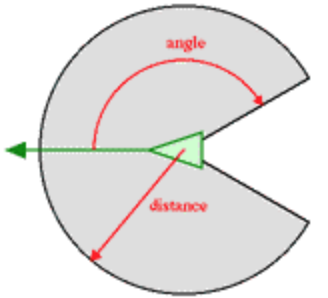
\includegraphics[width=\linewidth,height=0.5\textheight,keepaspectratio]{{../imgs/neighbourhood}.png}
        \end{columns}
    \end{frame}
    \subsection{Algoritmo}
    \begin{frame}
        \frametitle{Boids: Algoritmo}
        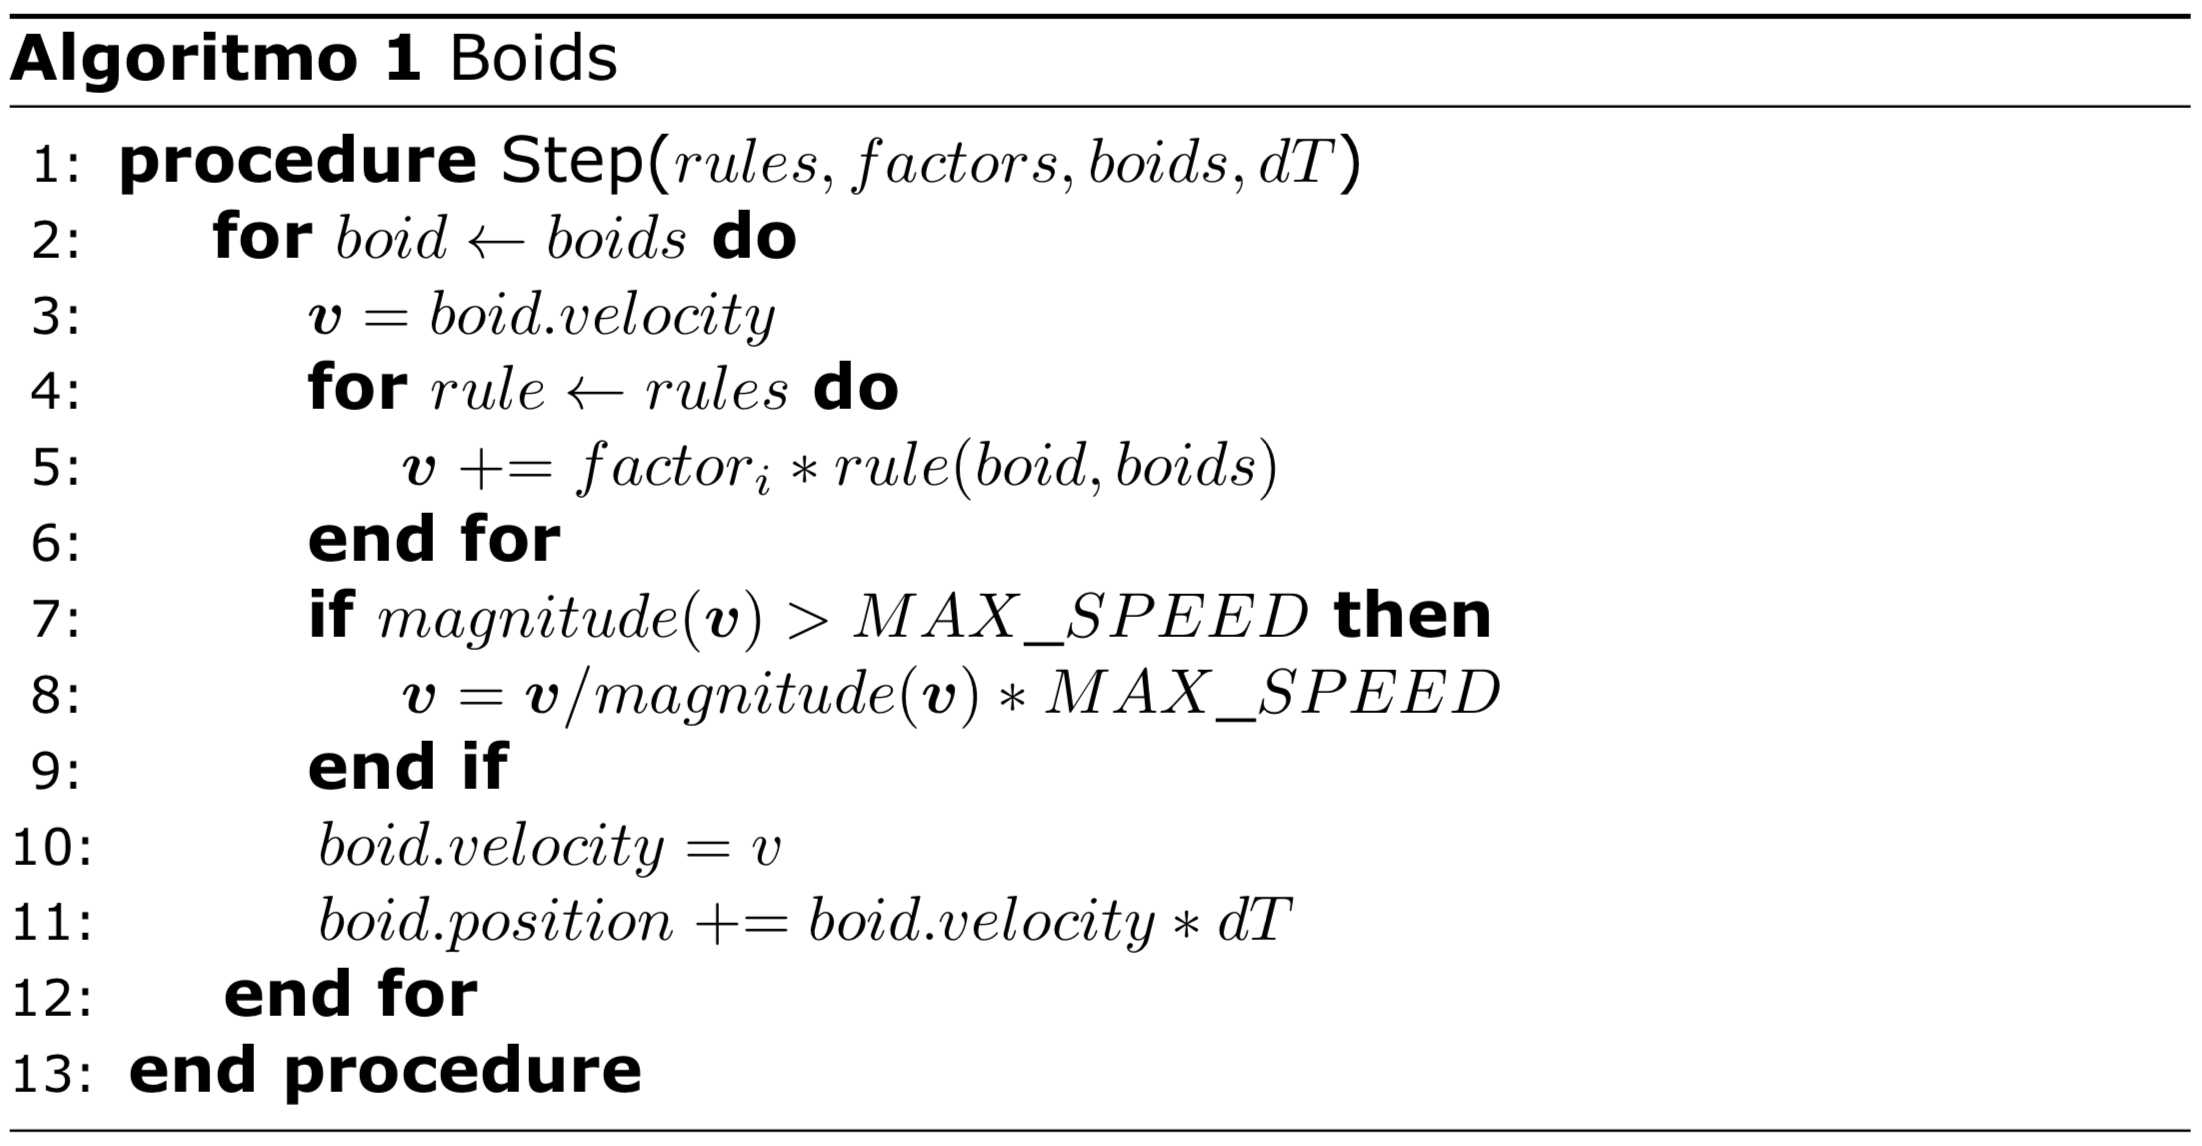
\includegraphics[width=\linewidth,height=\textheight,keepaspectratio]{{../imgs/algo_boids}.png}
    \end{frame}
    \subsection{Reglas básicas}

    \begin{frame}
        \frametitle{Regla: Alineamiento}
        \begin{columns}
            \column{0.7\textwidth}
            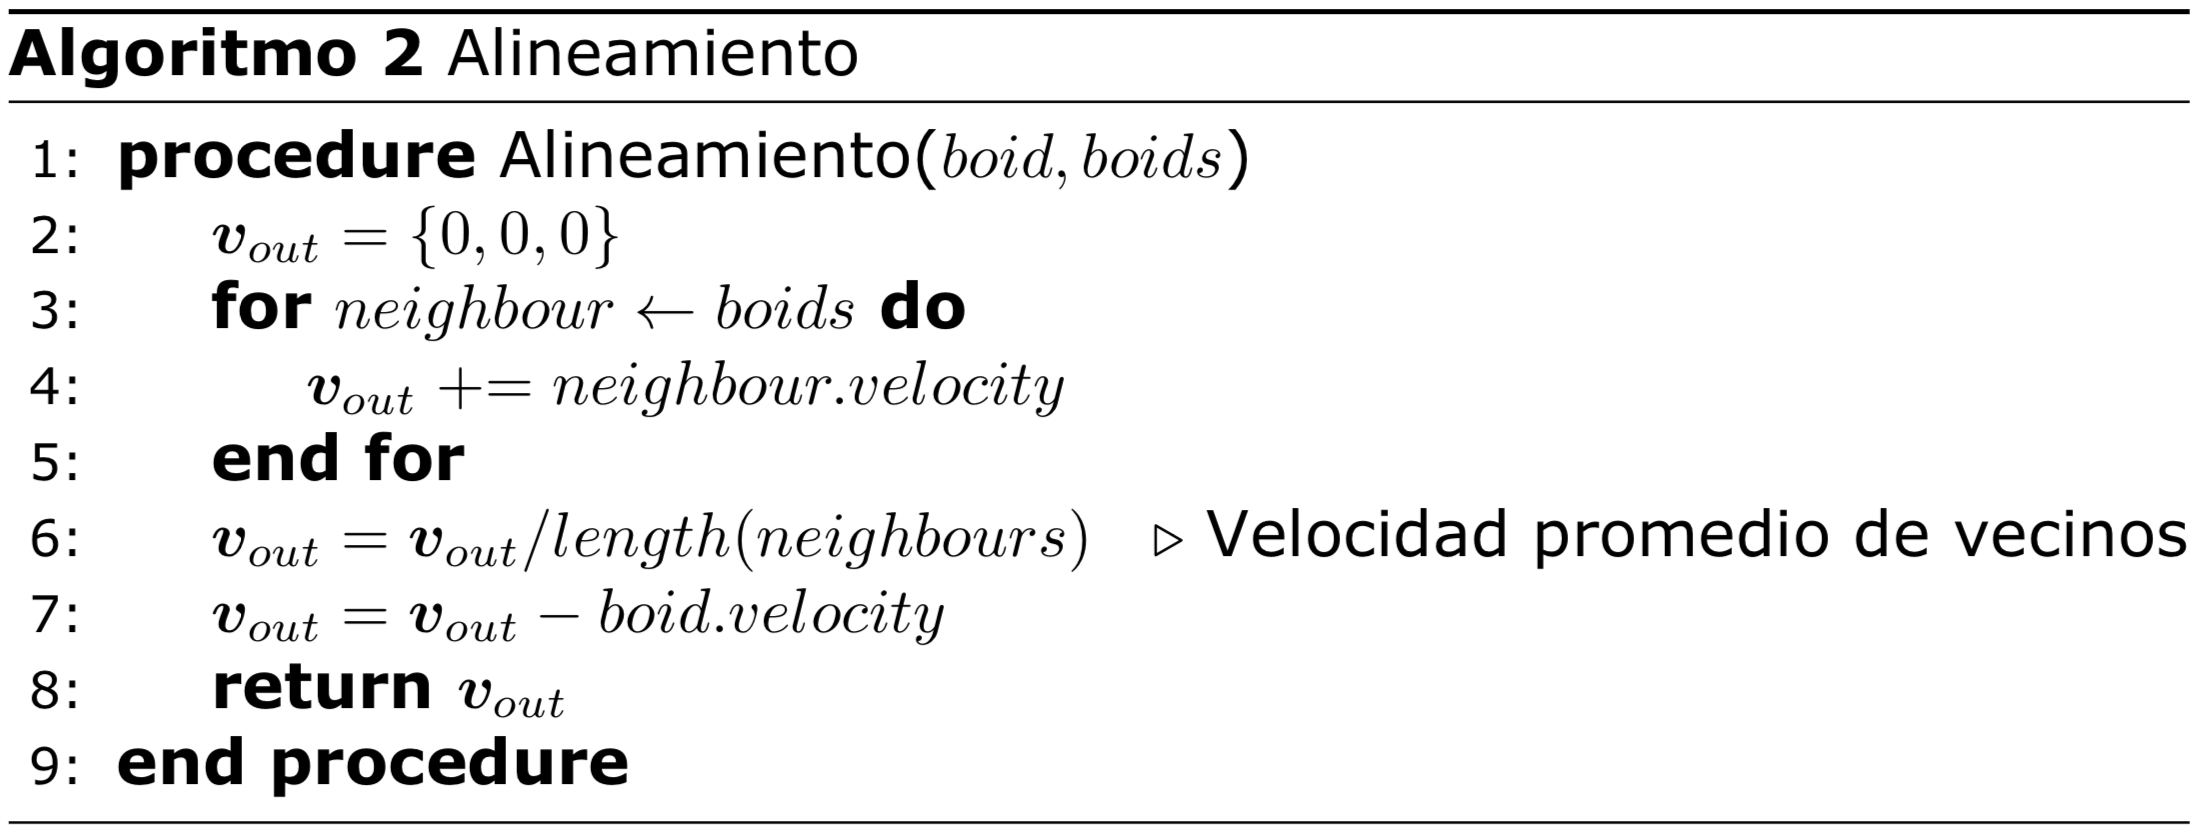
\includegraphics[width=\linewidth,height=\textheight,keepaspectratio]{{../imgs/algo_alignment}.png}
            \column{0.3\textwidth}
            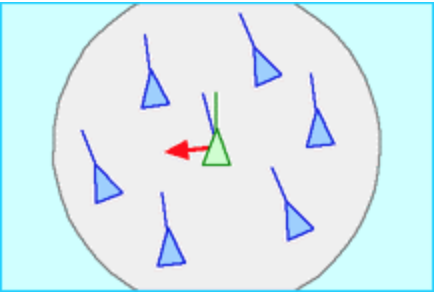
\includegraphics[width=\linewidth,height=\textheight,keepaspectratio]{{../imgs/rule_alignment}.png}
        \end{columns}
    \end{frame}

    \begin{frame}
        \frametitle{Regla: Separación}
        \begin{columns}
            \column{0.7\textwidth}
            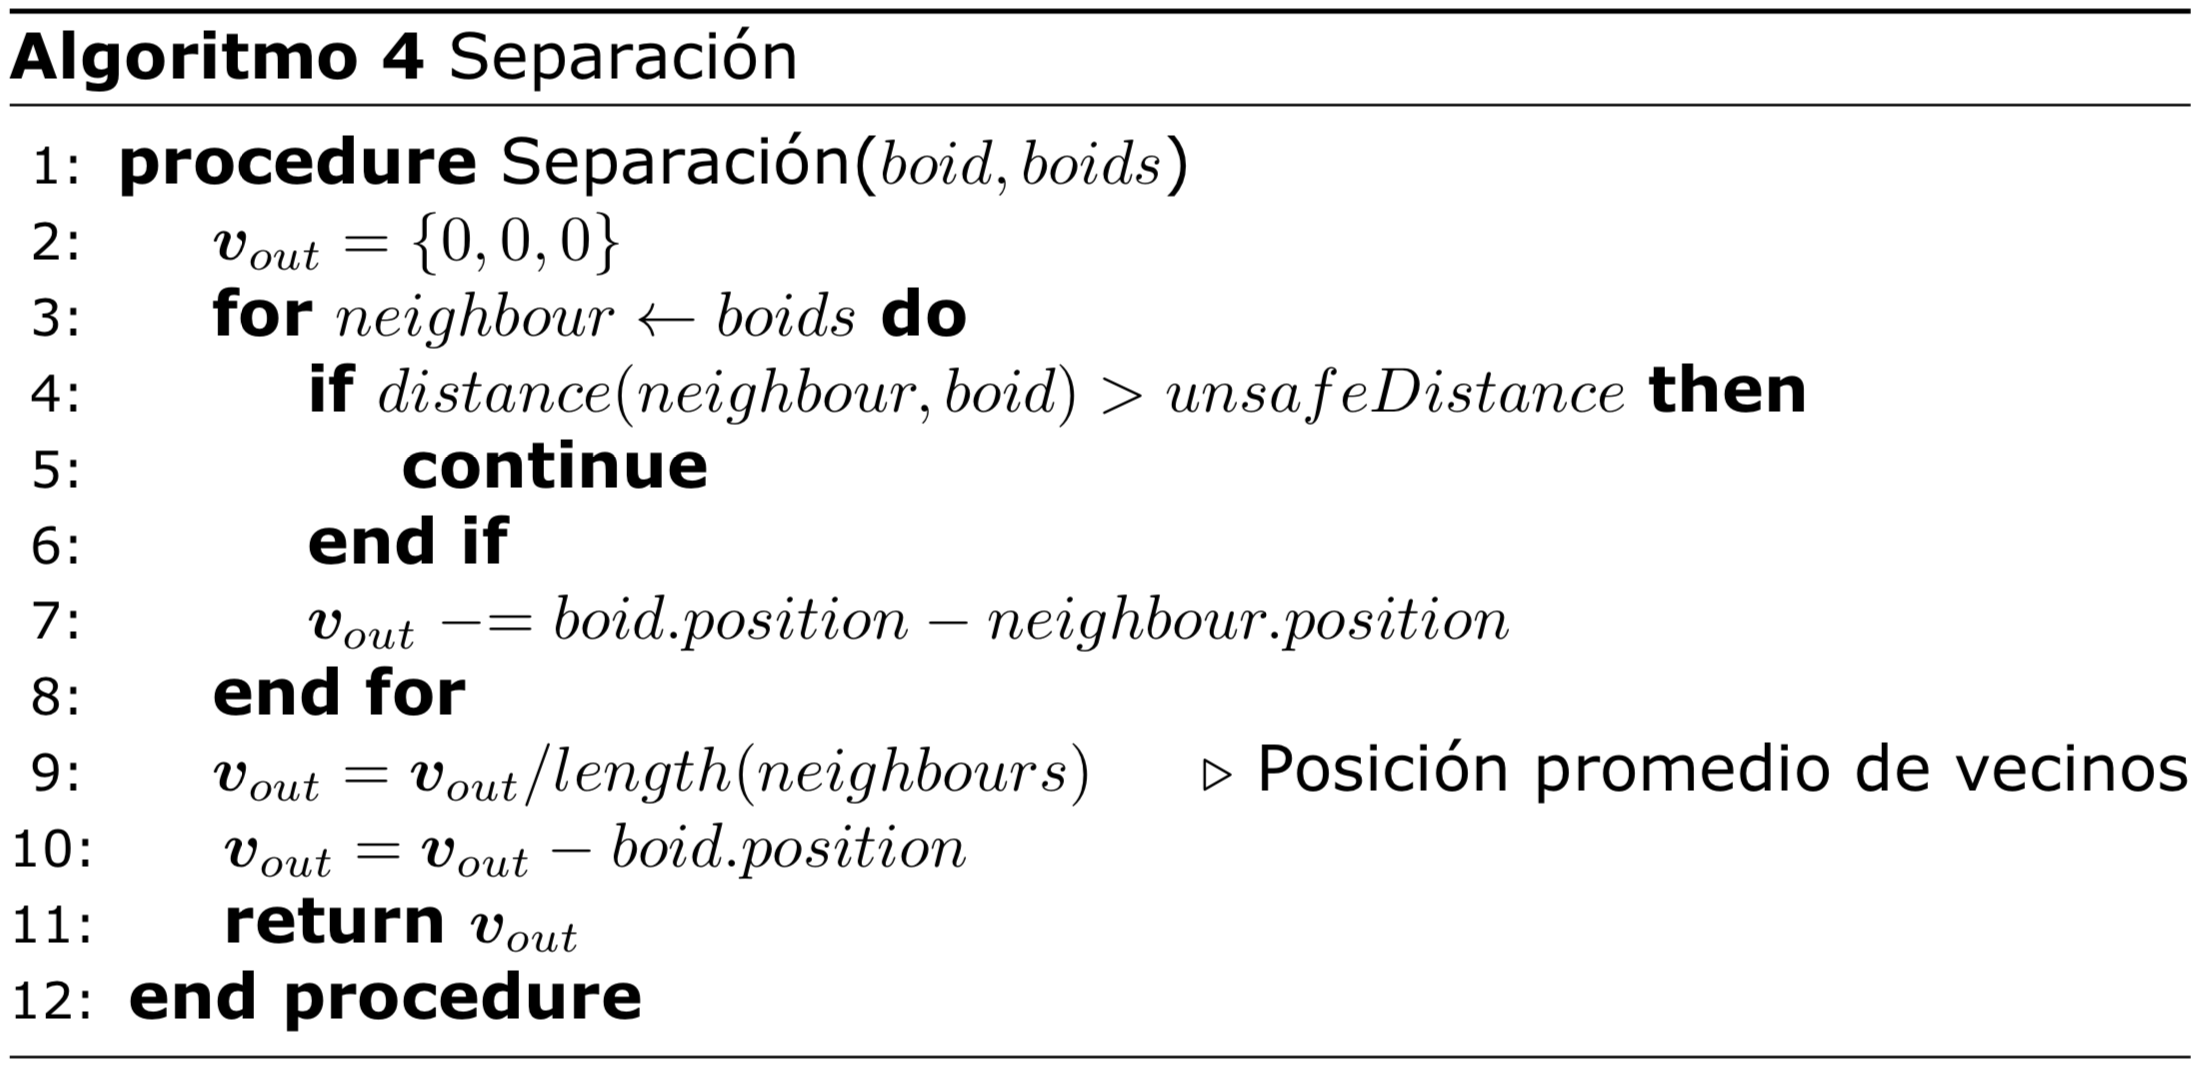
\includegraphics[width=\linewidth,height=\textheight,keepaspectratio]{{../imgs/algo_separation}.png}
            \column{0.3\textwidth}
            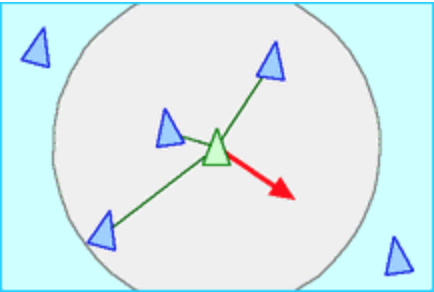
\includegraphics[width=\linewidth,height=\textheight,keepaspectratio]{{../imgs/rule_separation}.png}
        \end{columns}
    \end{frame}

    \begin{frame}
        \frametitle{Regla: Cohesión}
        \begin{columns}
            \column{0.7\textwidth}
            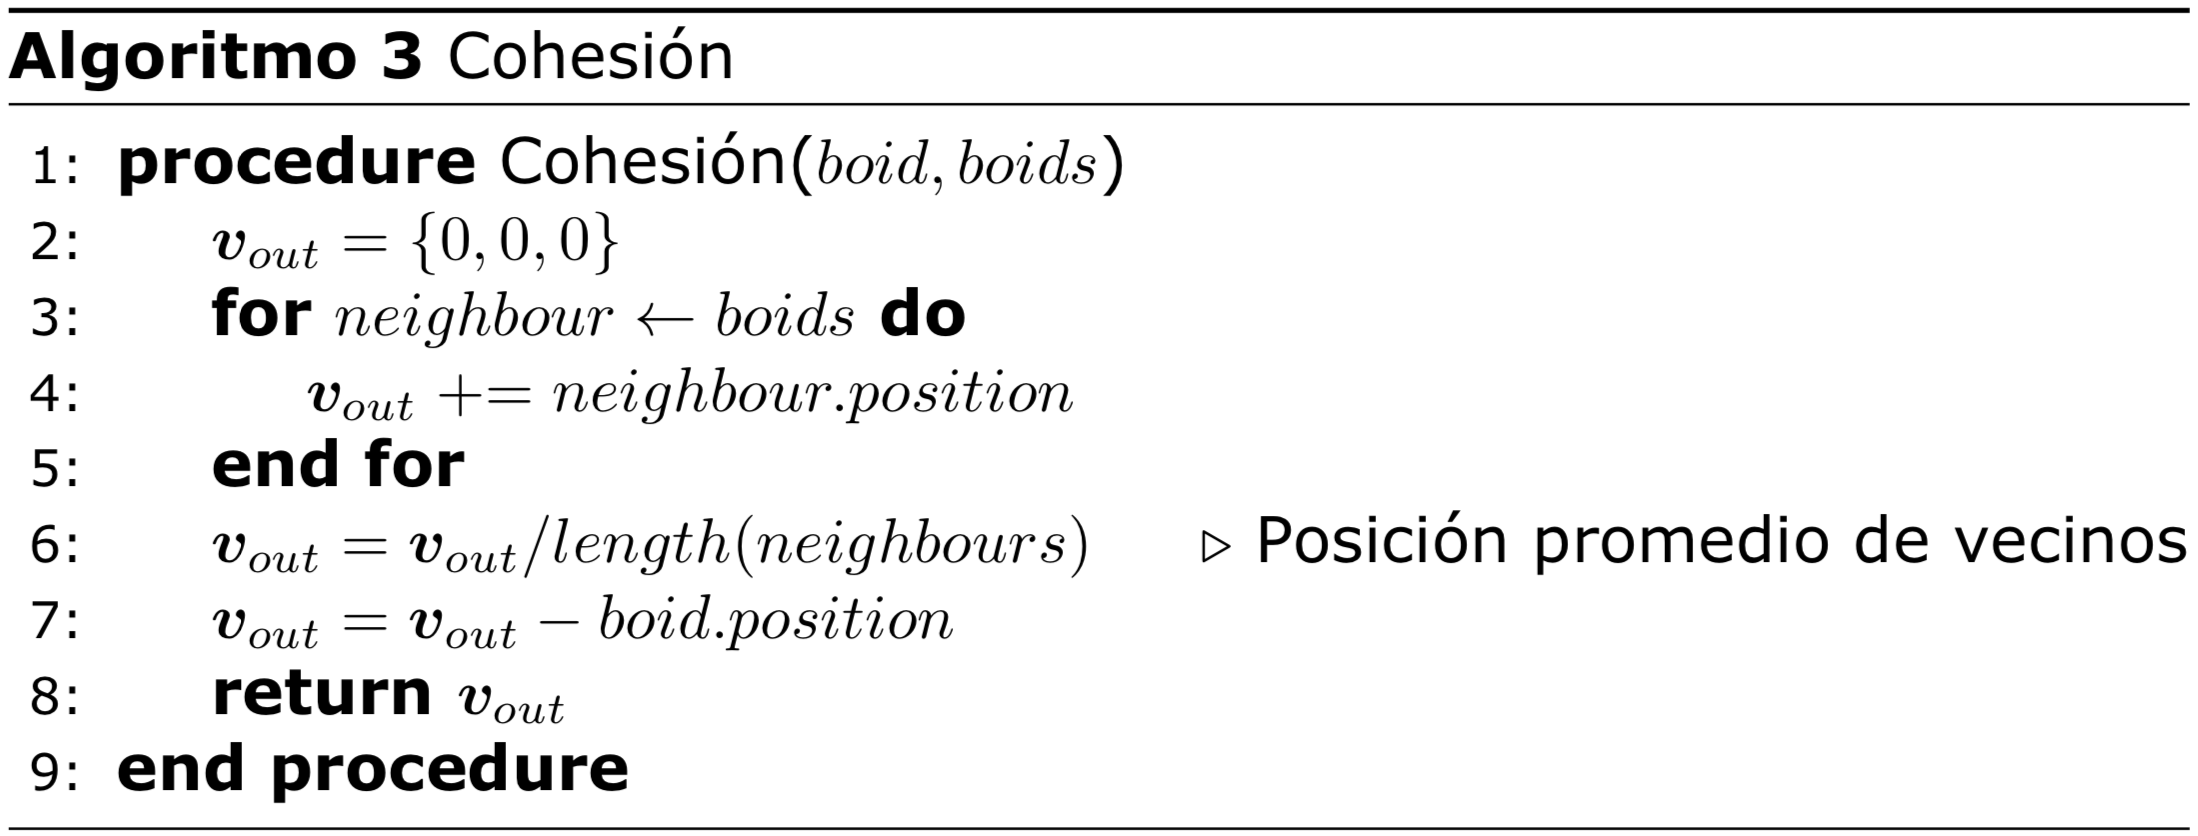
\includegraphics[width=\linewidth,height=\textheight,keepaspectratio]{{../imgs/algo_cohesion}.png}
            \column{0.3\textwidth}
            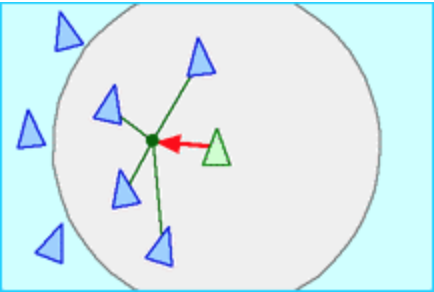
\includegraphics[width=\linewidth,height=\textheight,keepaspectratio]{{../imgs/rule_cohesion}.png}
        \end{columns}
    \end{frame}
    \subsection{Reglas extendidas}
    \begin{frame}
        \frametitle{Regla: Tendencia a}
        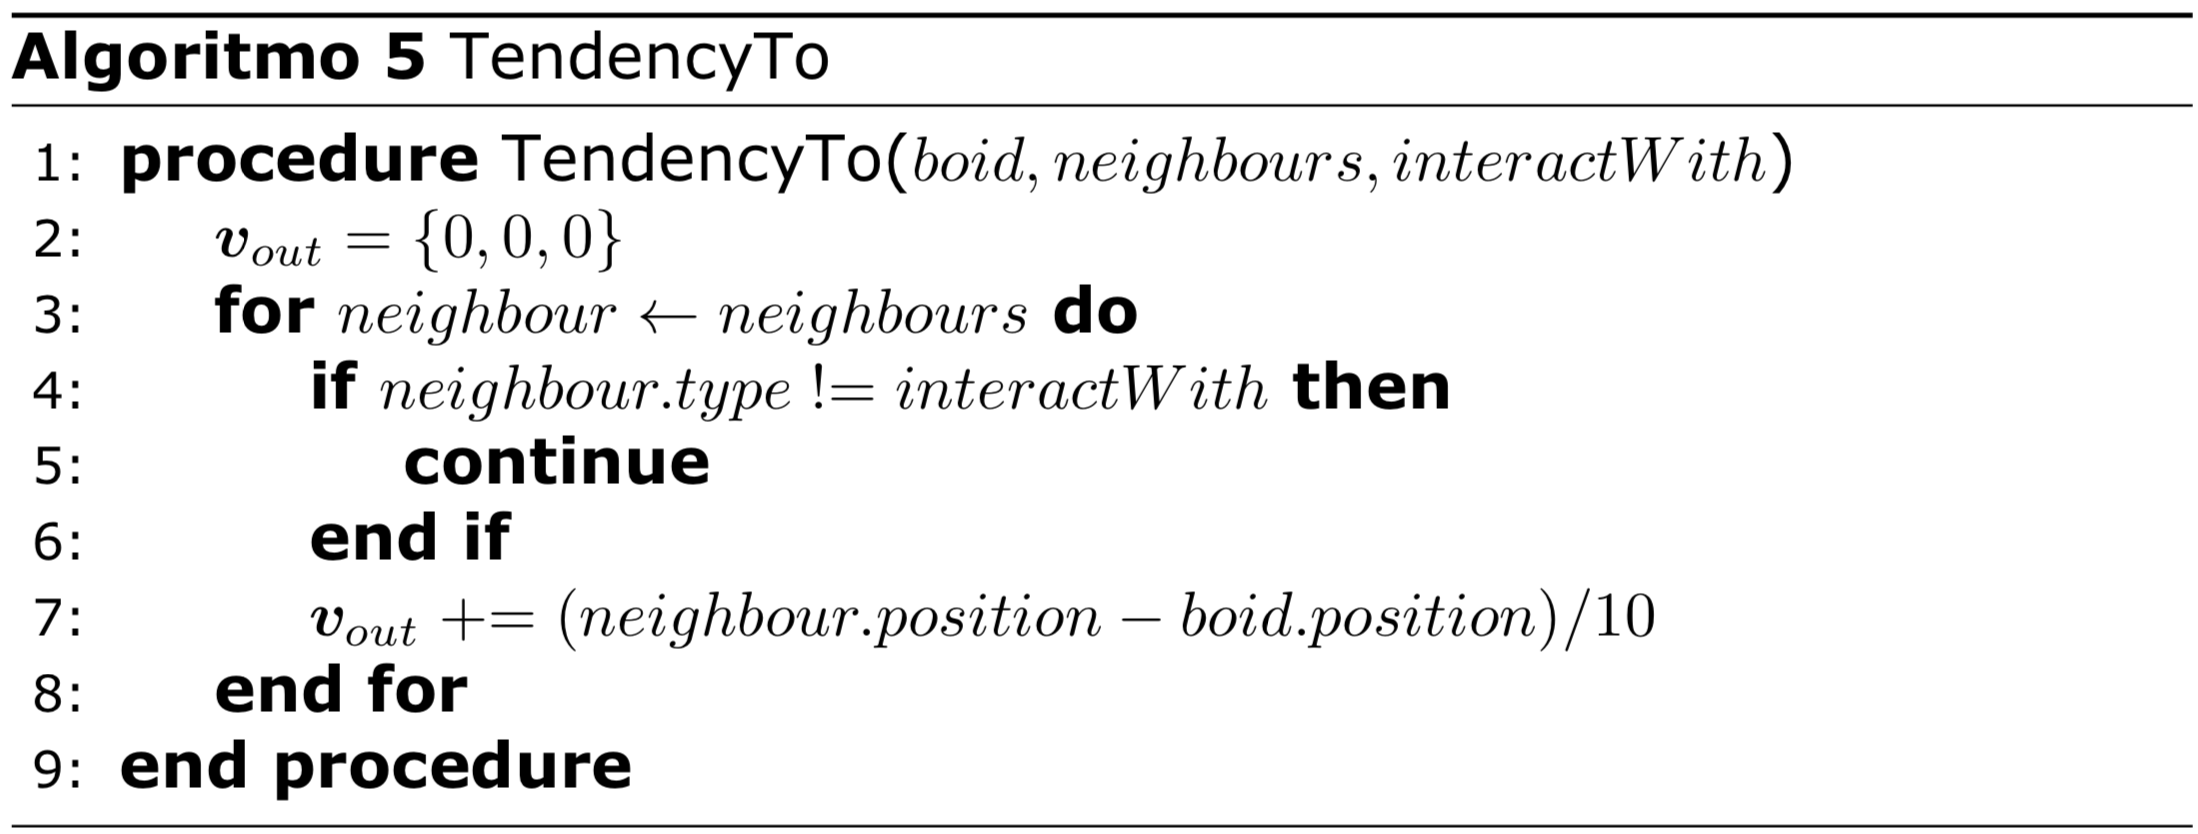
\includegraphics[width=\linewidth,height=\textheight,keepaspectratio]{{../imgs/algo_tendencyto}.png}
    \end{frame}

    \begin{frame}
        \frametitle{Regla: Frontera}
        \begin{center}
        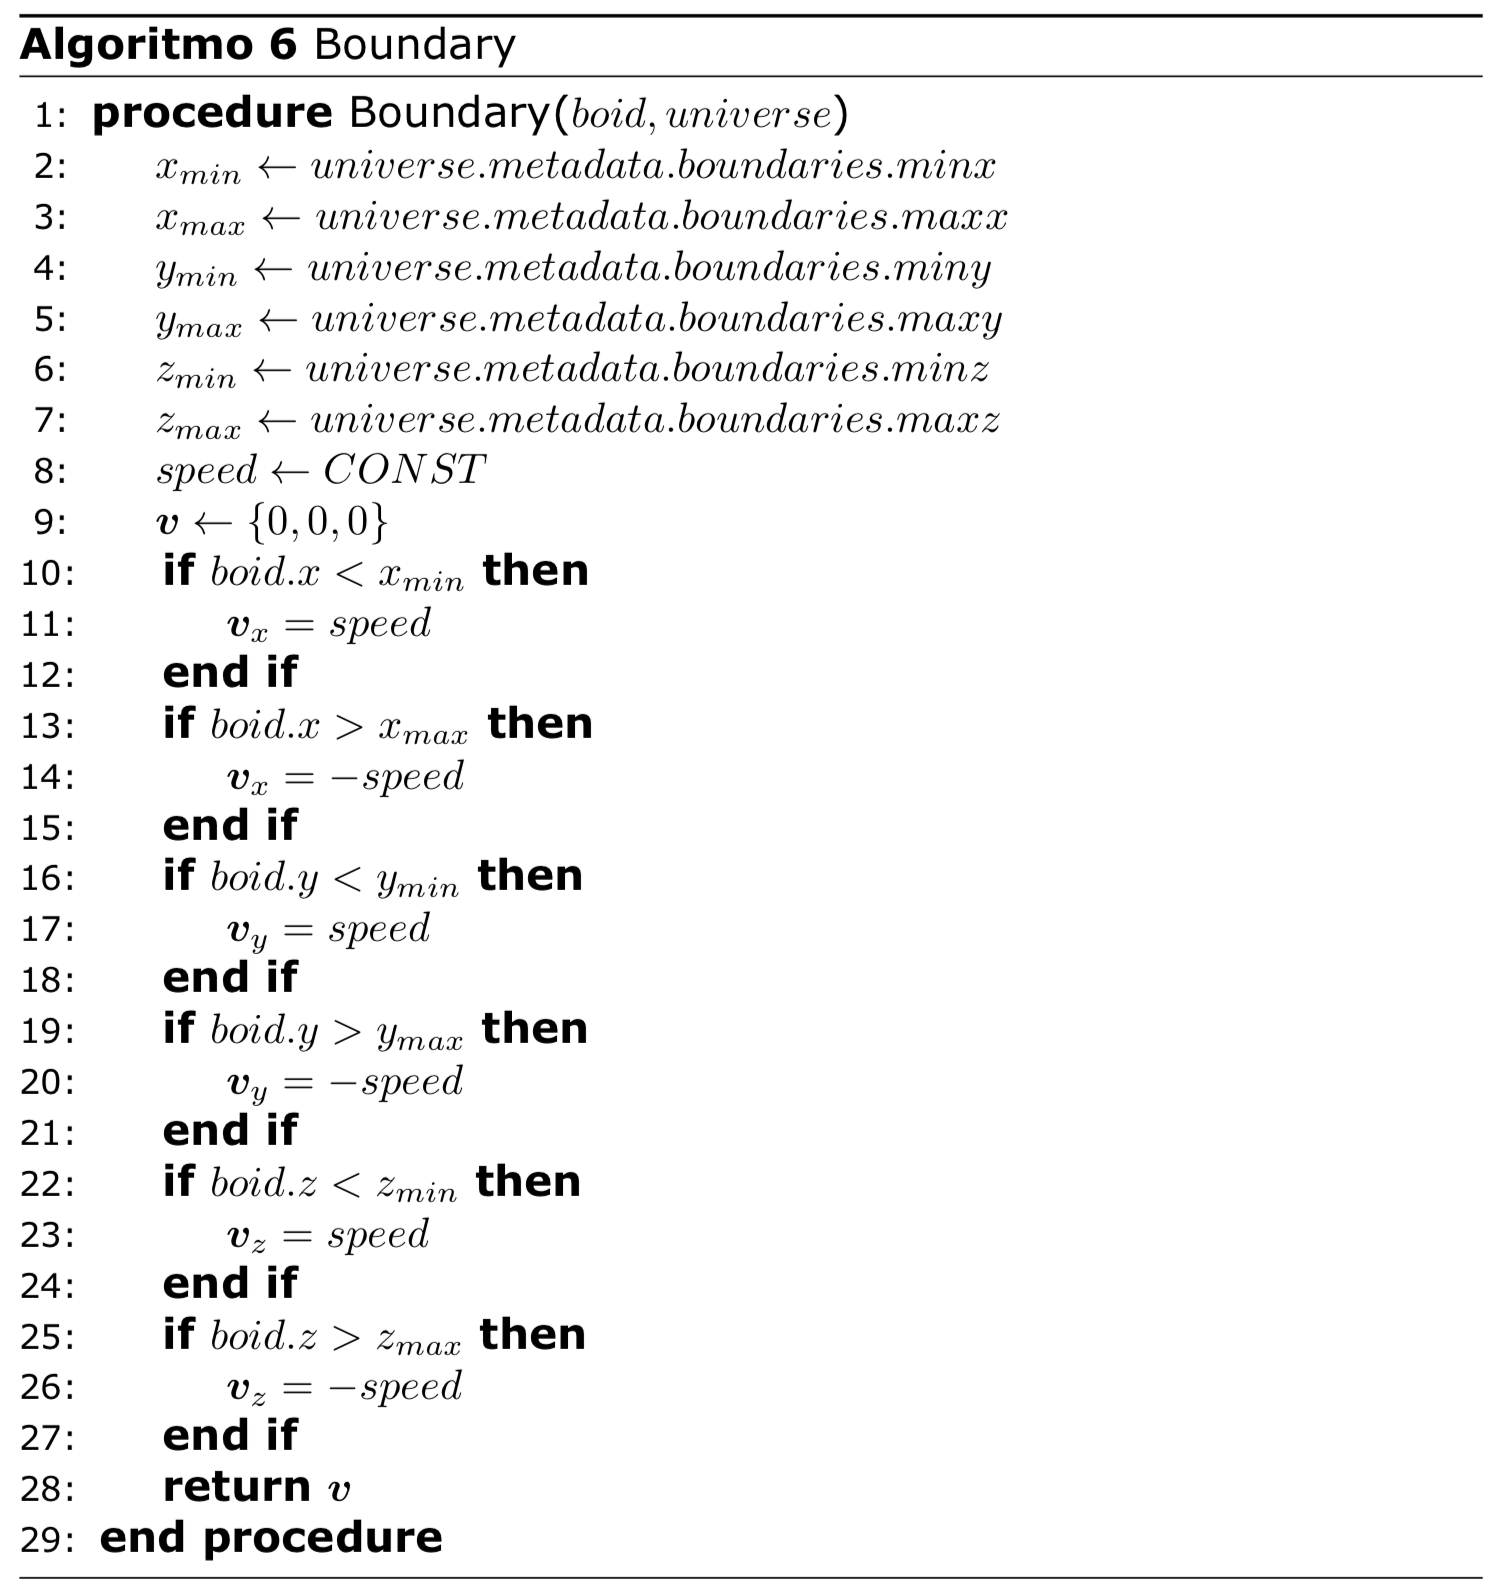
\includegraphics[width=\linewidth,height=0.9\textheight,keepaspectratio]{{../imgs/algo_boundary}.png}
        \end{center}
    \end{frame}

    \section{Implementación}
        \begin{frame}
            \frametitle{Implementación}
            \metroset{block=fill}
            \begin{block}{Lenguaje}
                Kotlin
            \end{block}
            \begin{block}{Visualización}
                Ovito
            \end{block}
            \begin{block}{Avance de simulación y animación}
                $\Delta t = \frac{1}{60}$ (s)
            \end{block}
        \end{frame}

        \begin{frame}
            \frametitle{Visualización: Color}
            \begin{columns}
                \column{0.5\textwidth}
                Color depende de la posición:
                \begin{itemize}
                    \item $R = 0.2 + (position.x / width) * 0.8$
                    \item $G = 0.2 + (position.y / height) * 0.8$
                    \item $B = 0.2 + (position.z / depth) * 0.8$
                \end{itemize}
                \column{0.5\textwidth}
                    TODO: Imagen de visualización
            \end{columns}
        \end{frame}


        \subsection{Código}

            \begin{frame}
                \frametitle{Entidades}
                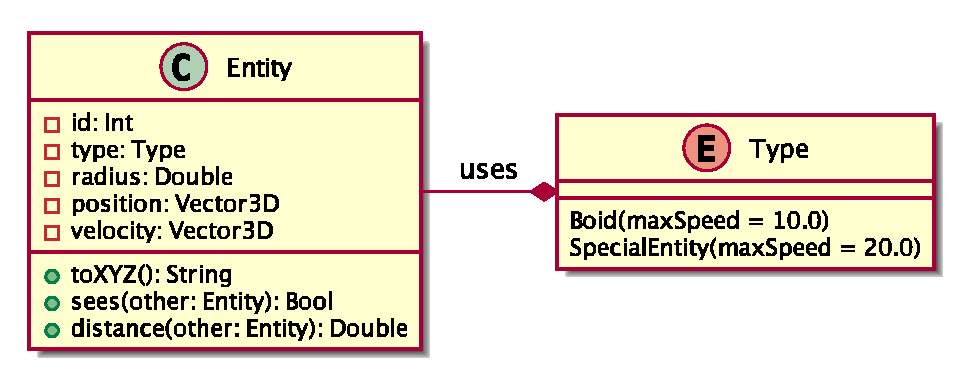
\includegraphics[width=\linewidth,height=\textheight,keepaspectratio]{{../imgs/entity}.eps}
            \end{frame}

            \begin{frame}
                \frametitle{Reglas}
                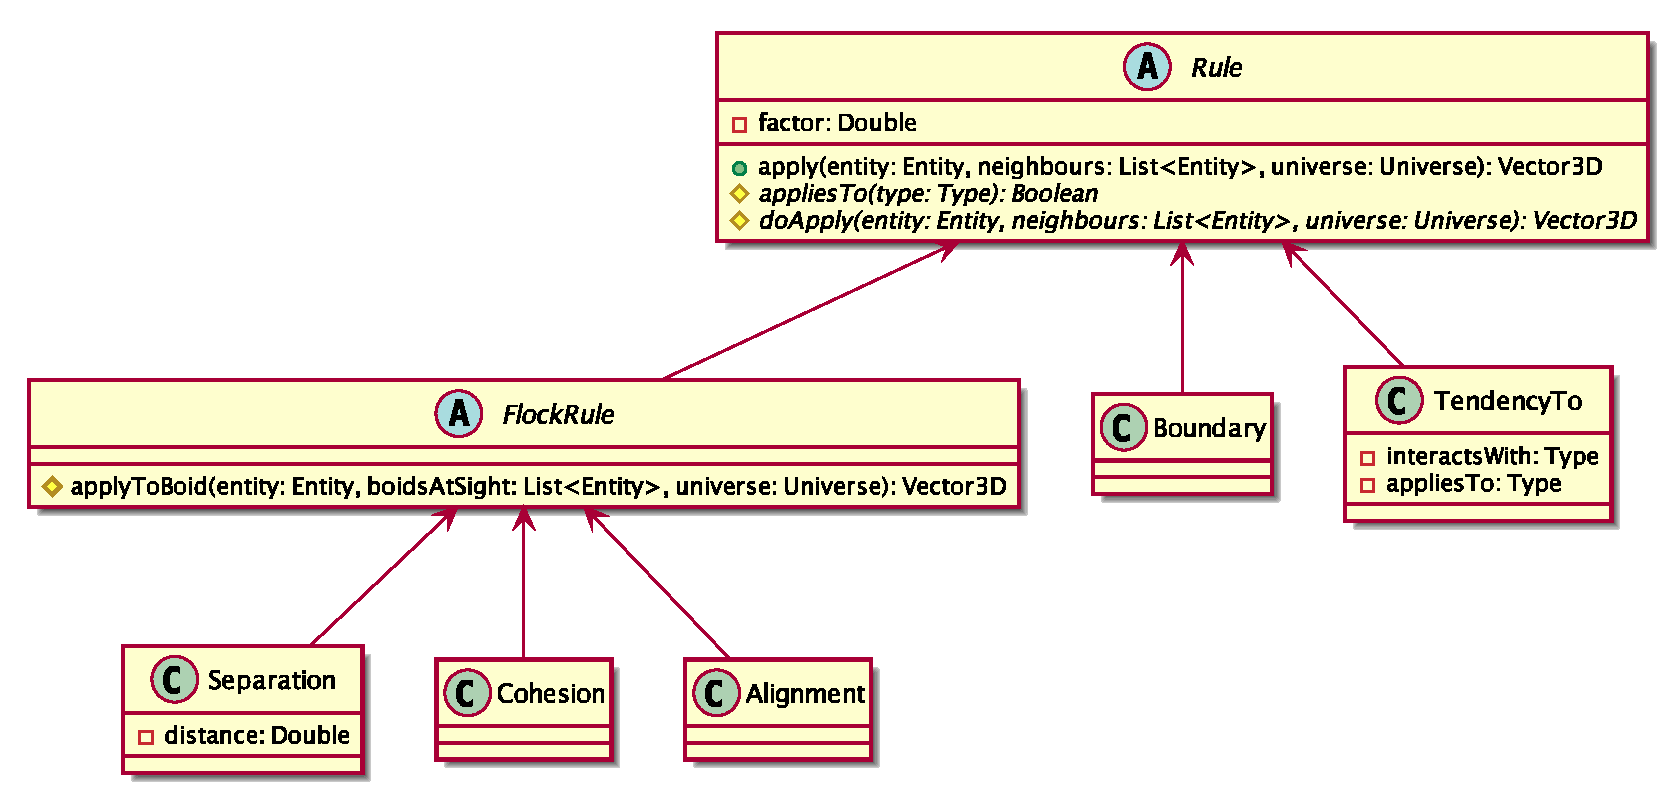
\includegraphics[width=\linewidth,height=\textheight,keepaspectratio]{{../imgs/rules}.eps}
            \end{frame}

            \begin{frame}
                \frametitle{Universo}
                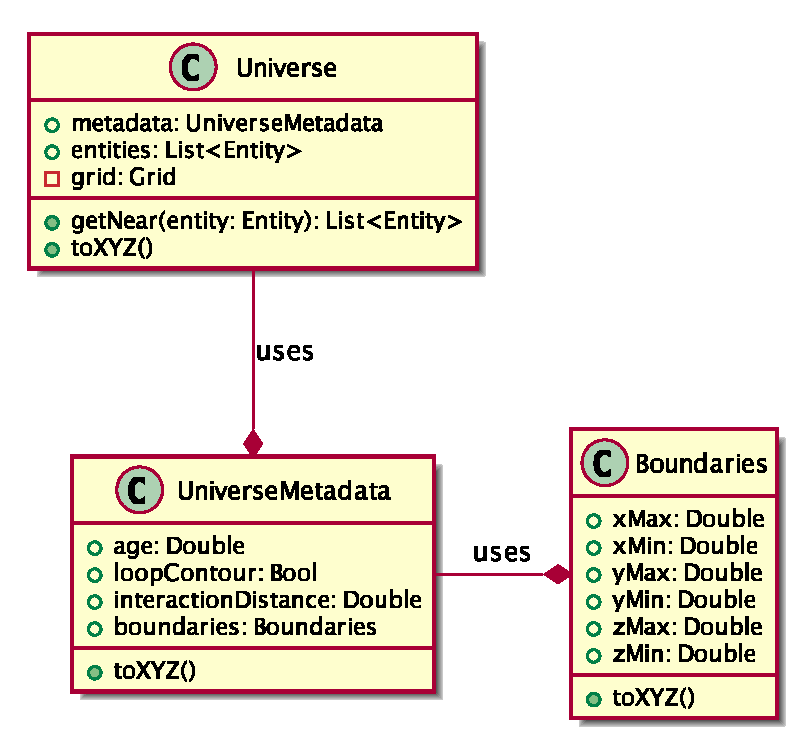
\includegraphics[width=\linewidth,height=\textheight,keepaspectratio]{{../imgs/universe}.eps}
            \end{frame}

            \begin{frame}
                \frametitle{Grilla}
                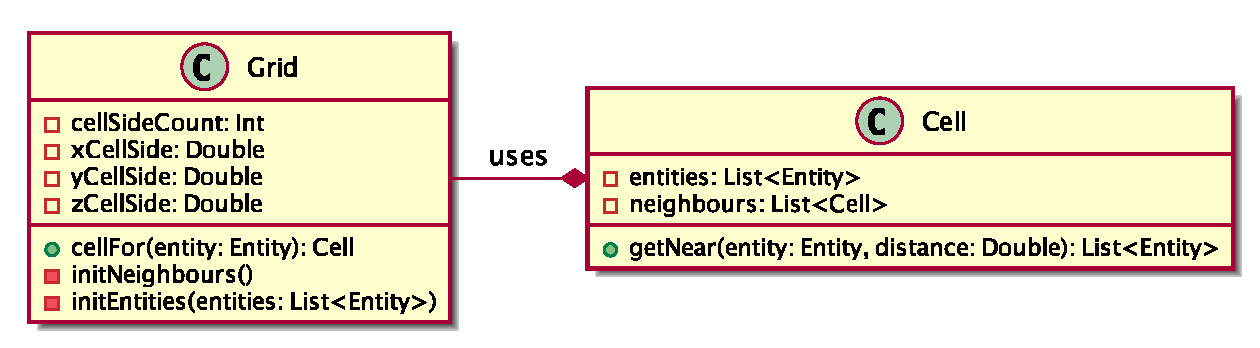
\includegraphics[width=\linewidth,height=\textheight,keepaspectratio]{{../imgs/grid}.eps}
            \end{frame}

            \begin{frame}
                \frametitle{Simulación}
                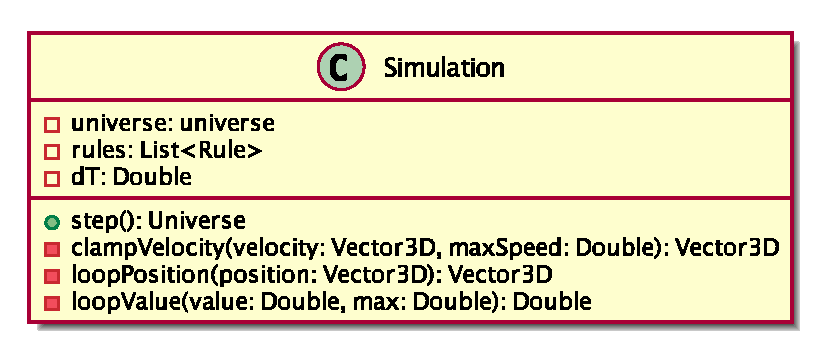
\includegraphics[width=\linewidth,height=\textheight,keepaspectratio]{{../imgs/simulation}.eps}
            \end{frame}

    \section{Resultados}
        \begin{frame}
            \frametitle{Parámetros de simulación}
            \metroset{block=fill}
            \begin{block}{Tamaño del universo}
                32m x 32m x 32m
            \end{block}
            \begin{block}{Condiciones de contorno}
                habilitadas
            \end{block}
            \begin{block}{Cantidad de boids}
                1024
            \end{block}
            \begin{block}{Cantidad de especiales}
                0
            \end{block}
            \begin{block}{Distancia de interacción}
                2m
            \end{block}
        \end{frame}
        \begin{frame}
            \frametitle{Parámetros de simulación}
            \metroset{block=fill}
            \begin{block}{Radio: boids}
                0.1m
            \end{block}
            \begin{block}{Radio: especiales}
                1.0m
            \end{block}
            \begin{block}{Velocidad máxima: boids}
                32 m/s
            \end{block}
            \begin{block}{Velocidad máxima: especiales}
                64 m/s
            \end{block}
        \end{frame}

        \begin{frame}
            \frametitle{Reglas: Factores}
            \metroset{block=fill}
            \begin{block}{Alineamiento}
                0.25
            \end{block}
            \begin{block}{Cohesión}
                0.25
            \end{block}
            \begin{block}{Separación}
                0.25
            \end{block}
            \begin{block}{Tendencia: Boid a Especial}
                -0.25
            \end{block}
            \begin{block}{Tendencia: Especial a Boid}
                0.25
            \end{block}
        \end{frame}
        \begin{frame}
            \frametitle{Polarización: Alineamiento}
            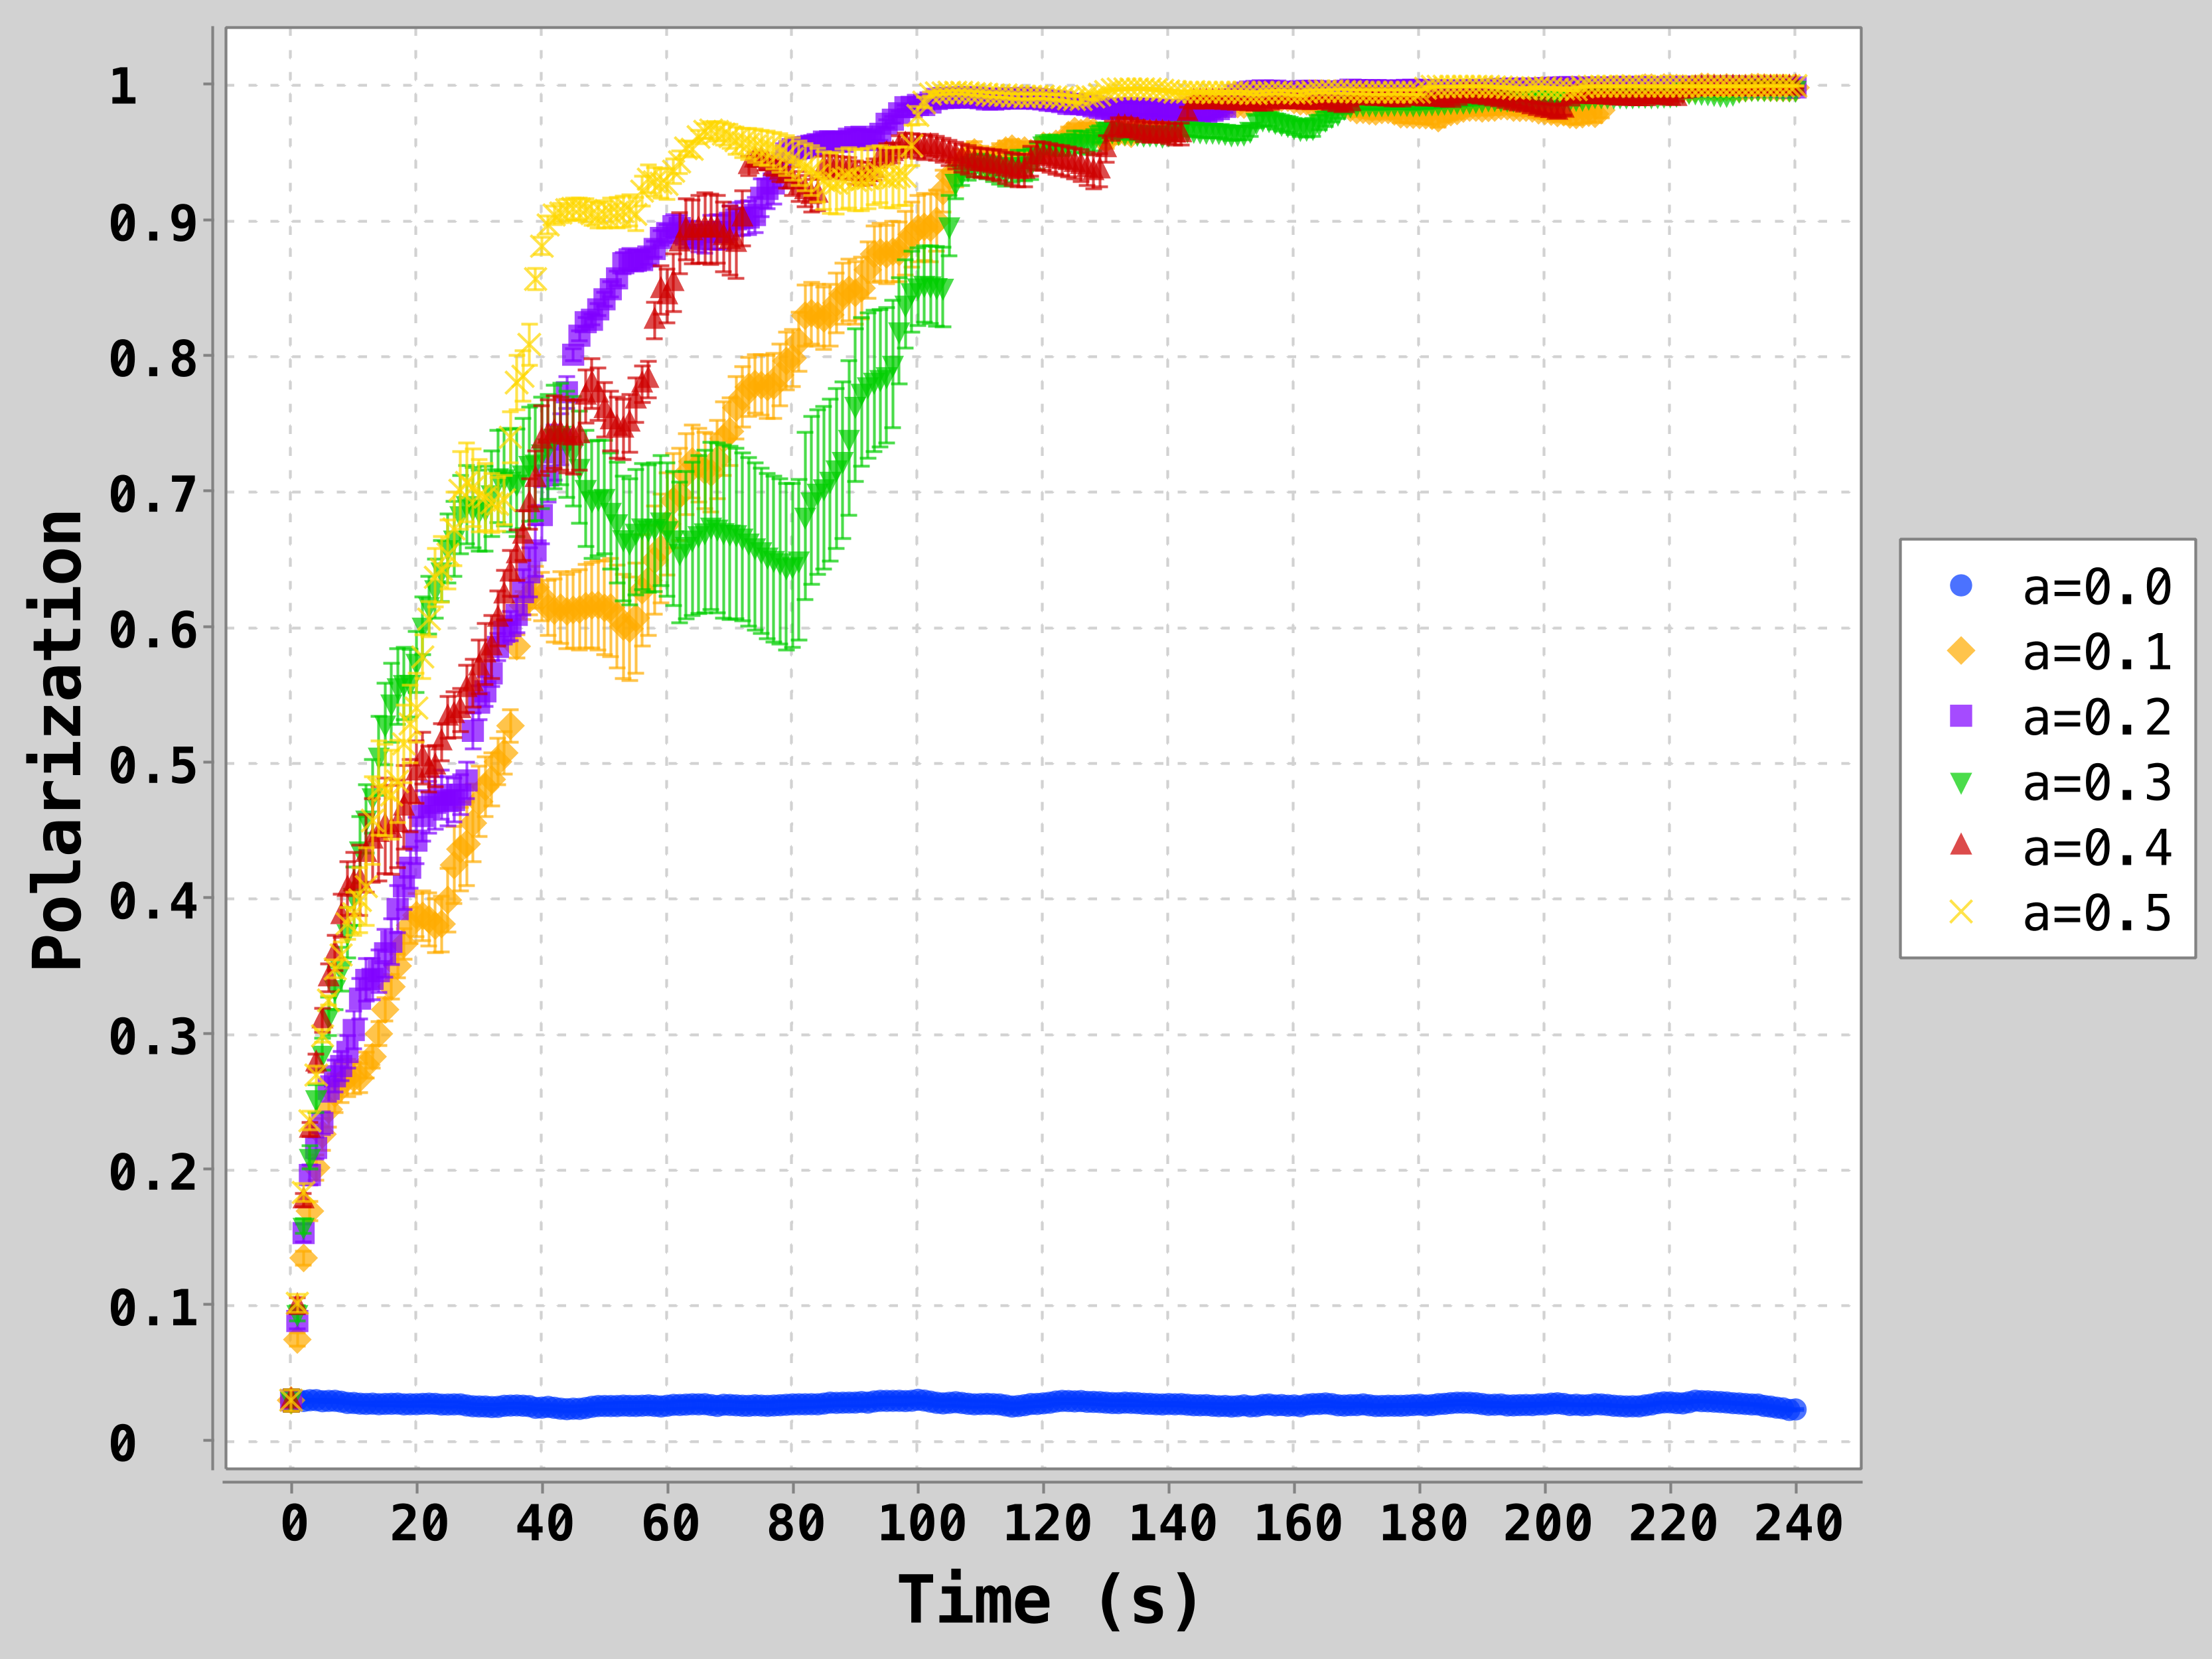
\includegraphics[width=\linewidth,height=\textheight,keepaspectratio]{{../imgs/polarization_a}.png}
        \end{frame}
        \begin{frame}
            \frametitle{Polarización: Cohesión}
            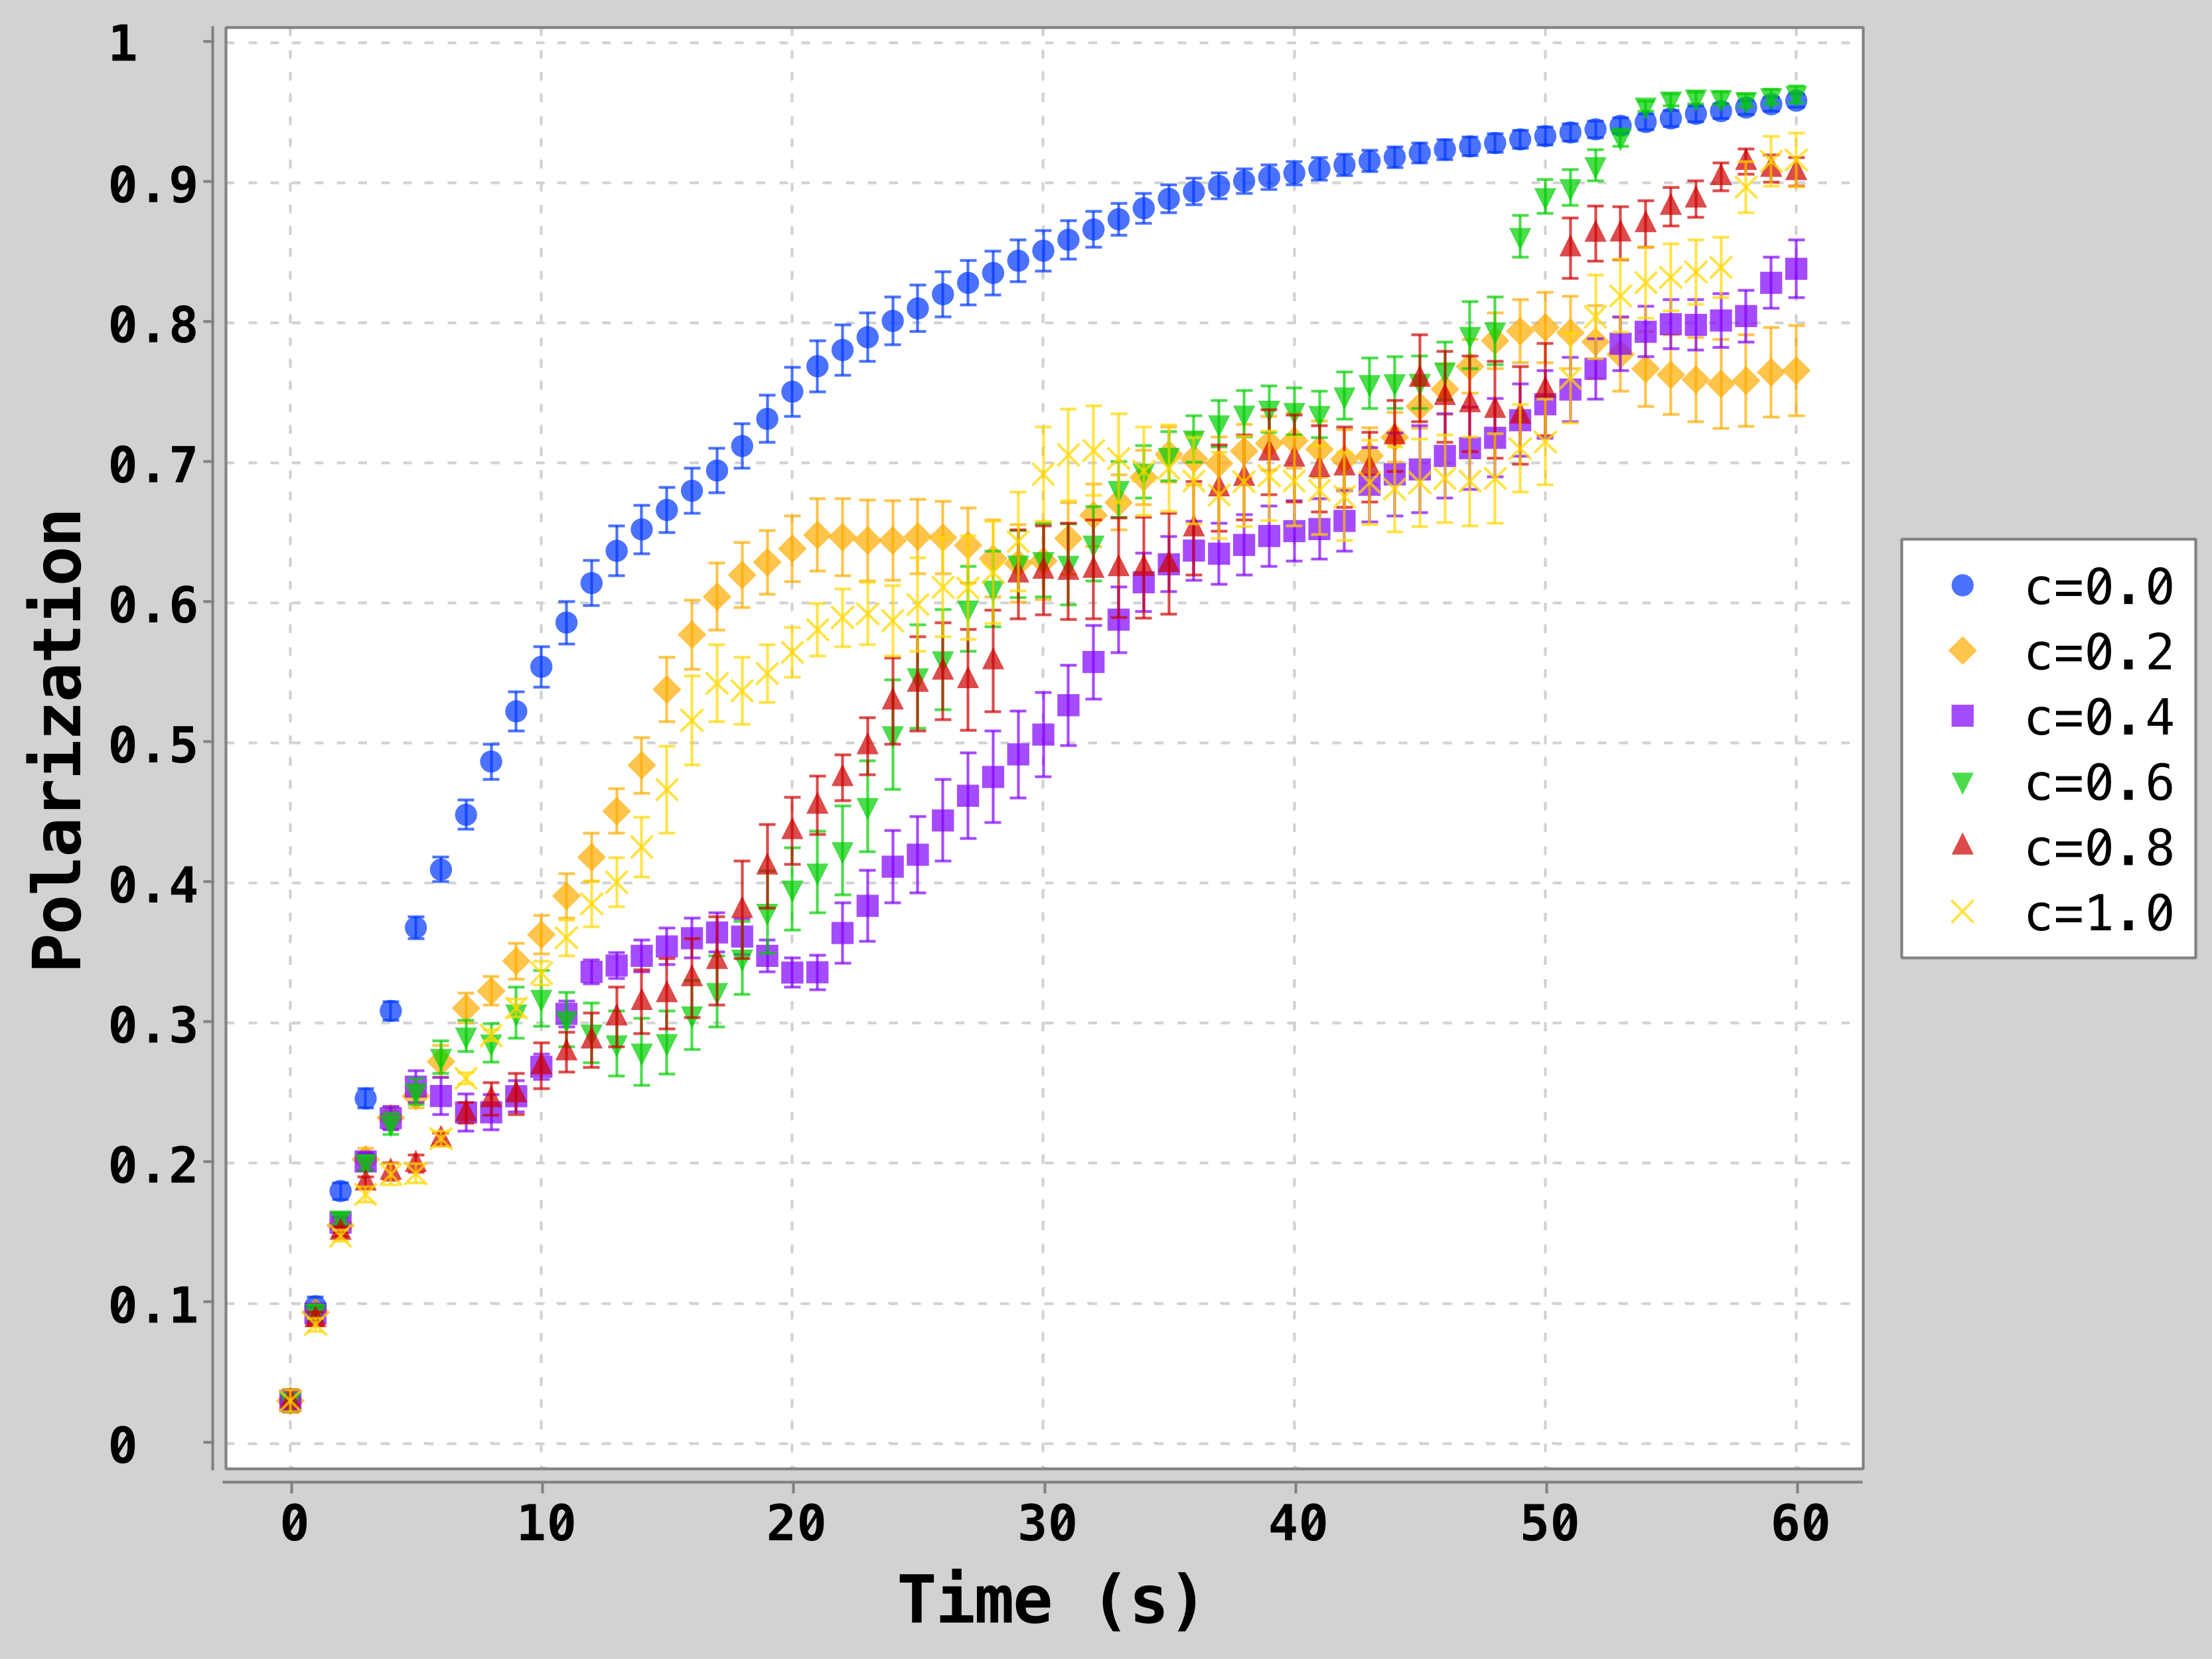
\includegraphics[width=\linewidth,height=\textheight,keepaspectratio]{{../imgs/polarization_c}.png}
        \end{frame}
        \begin{frame}
            \frametitle{Polarización: Separación}
            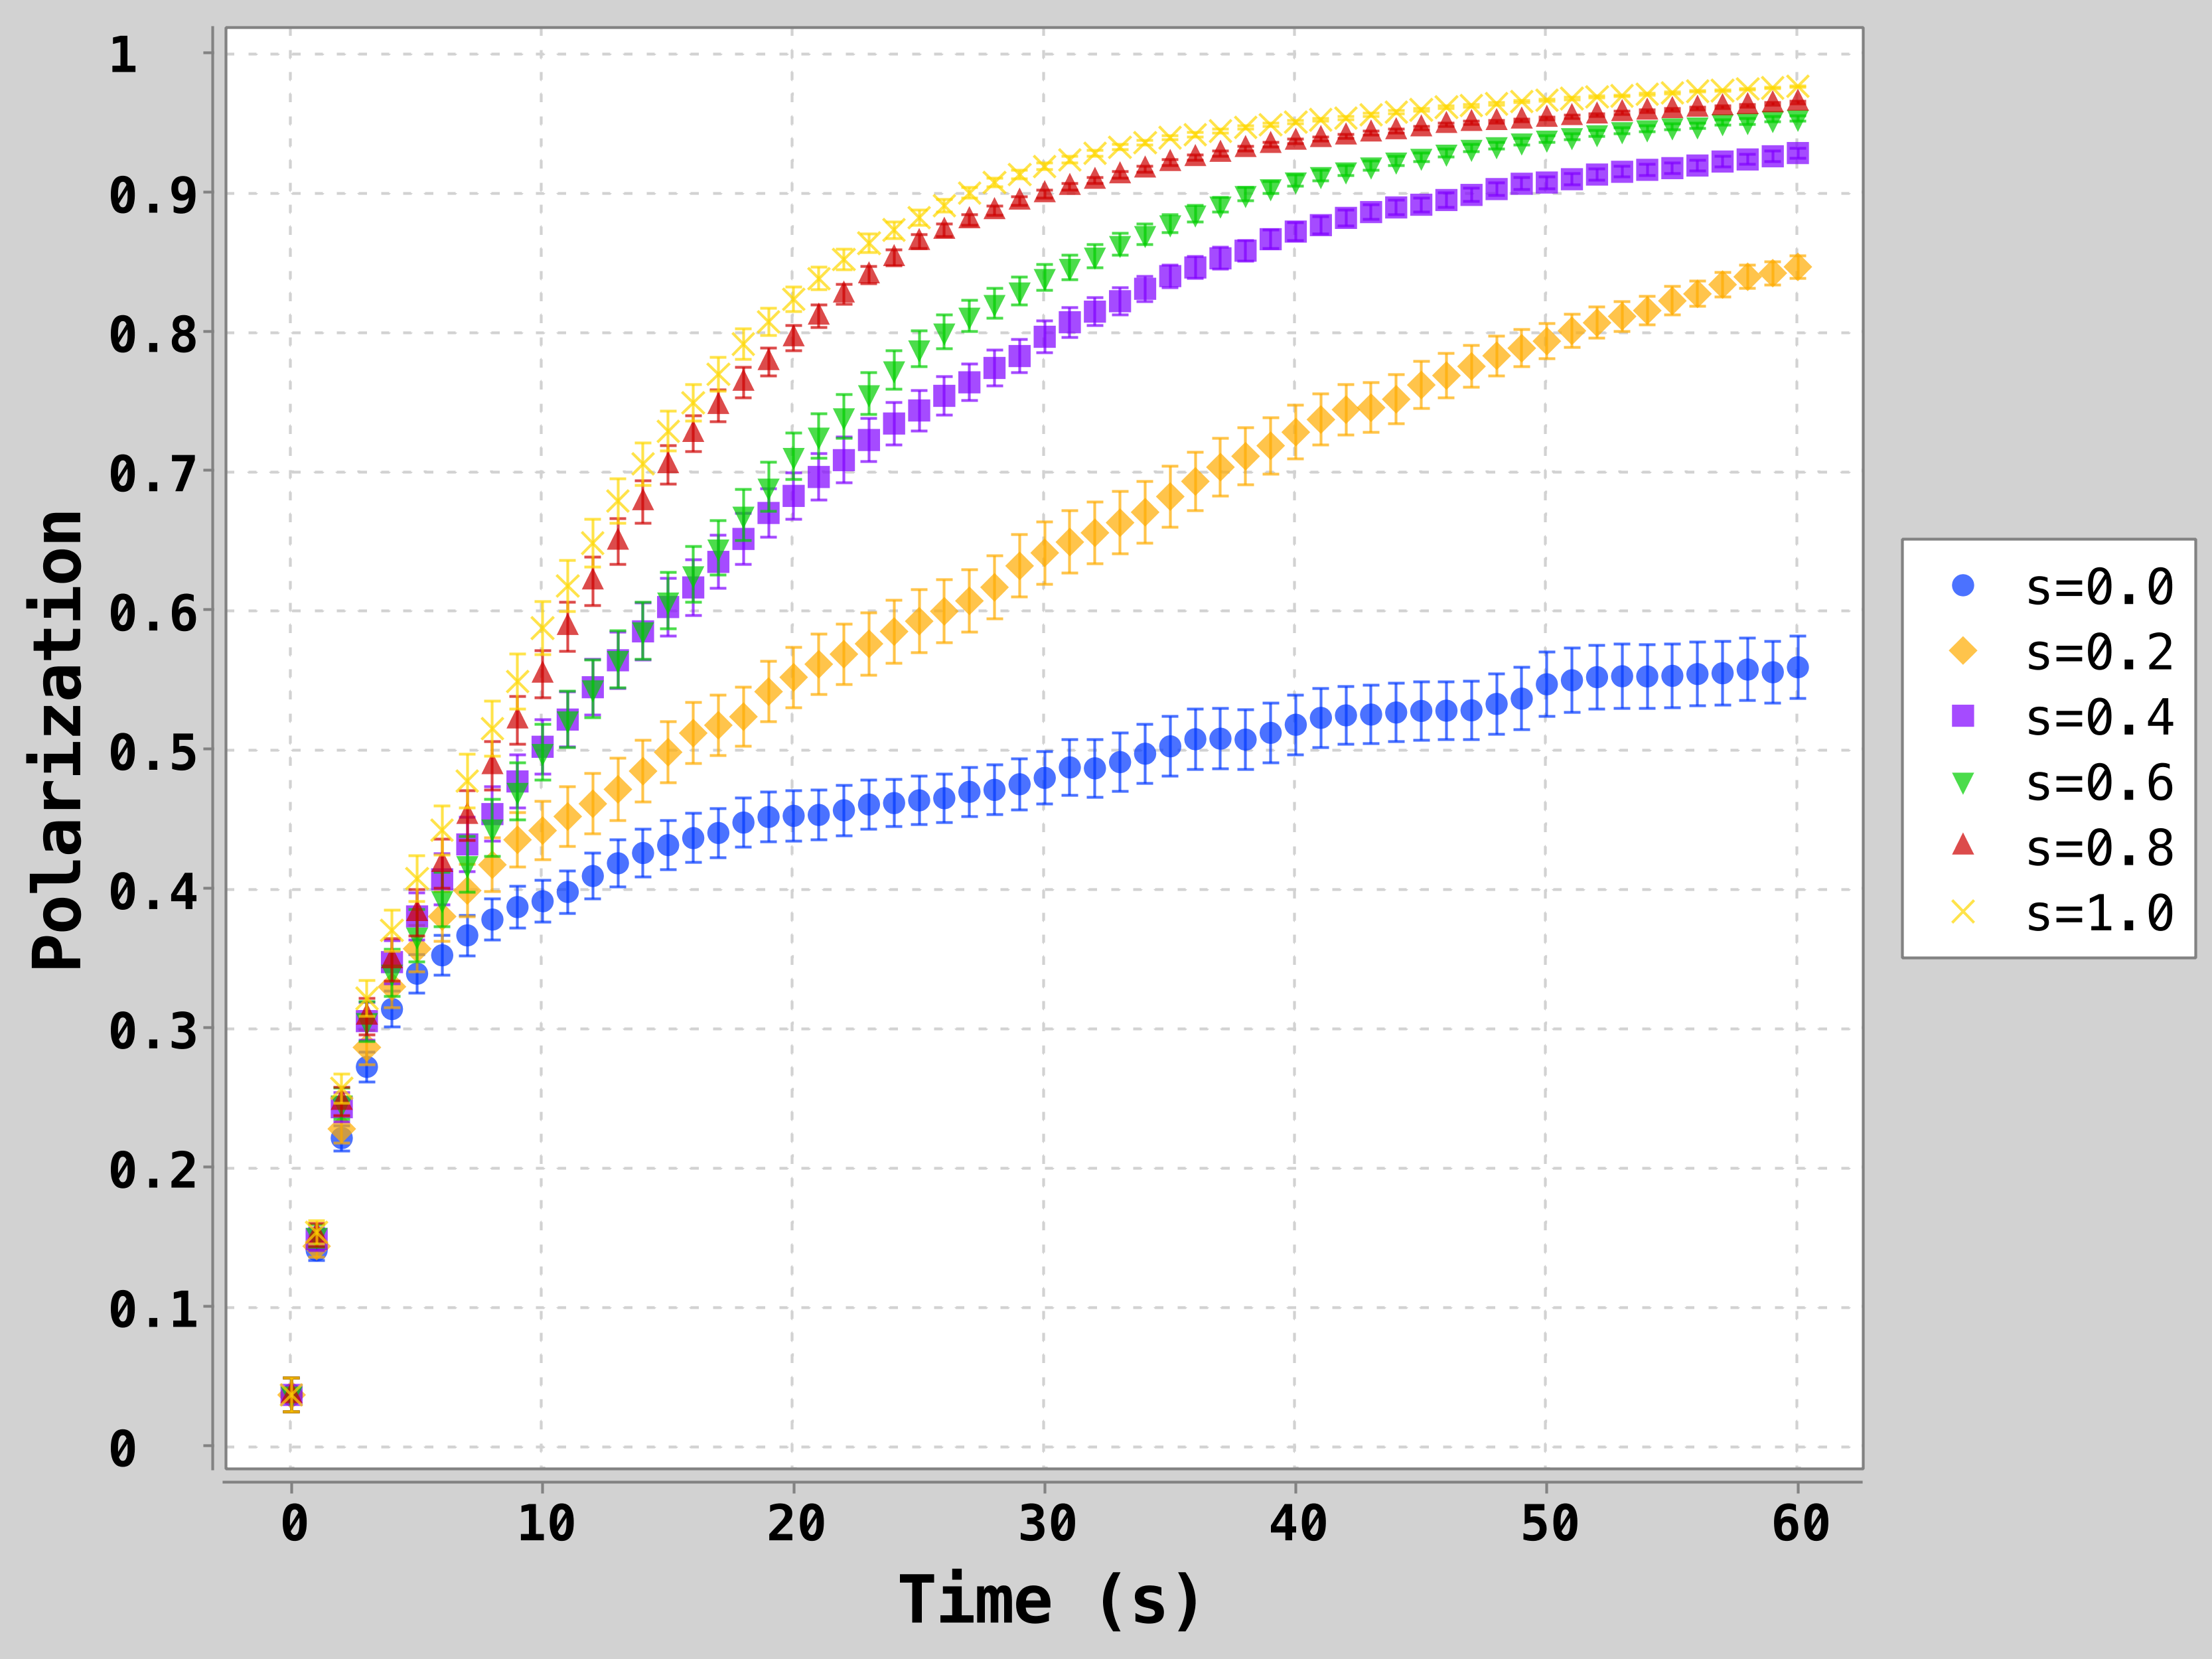
\includegraphics[width=\linewidth,height=\textheight,keepaspectratio]{{../imgs/polarization_s}.png}
        \end{frame}
        \begin{frame}
            \frametitle{Polarización: Tendencia a}
            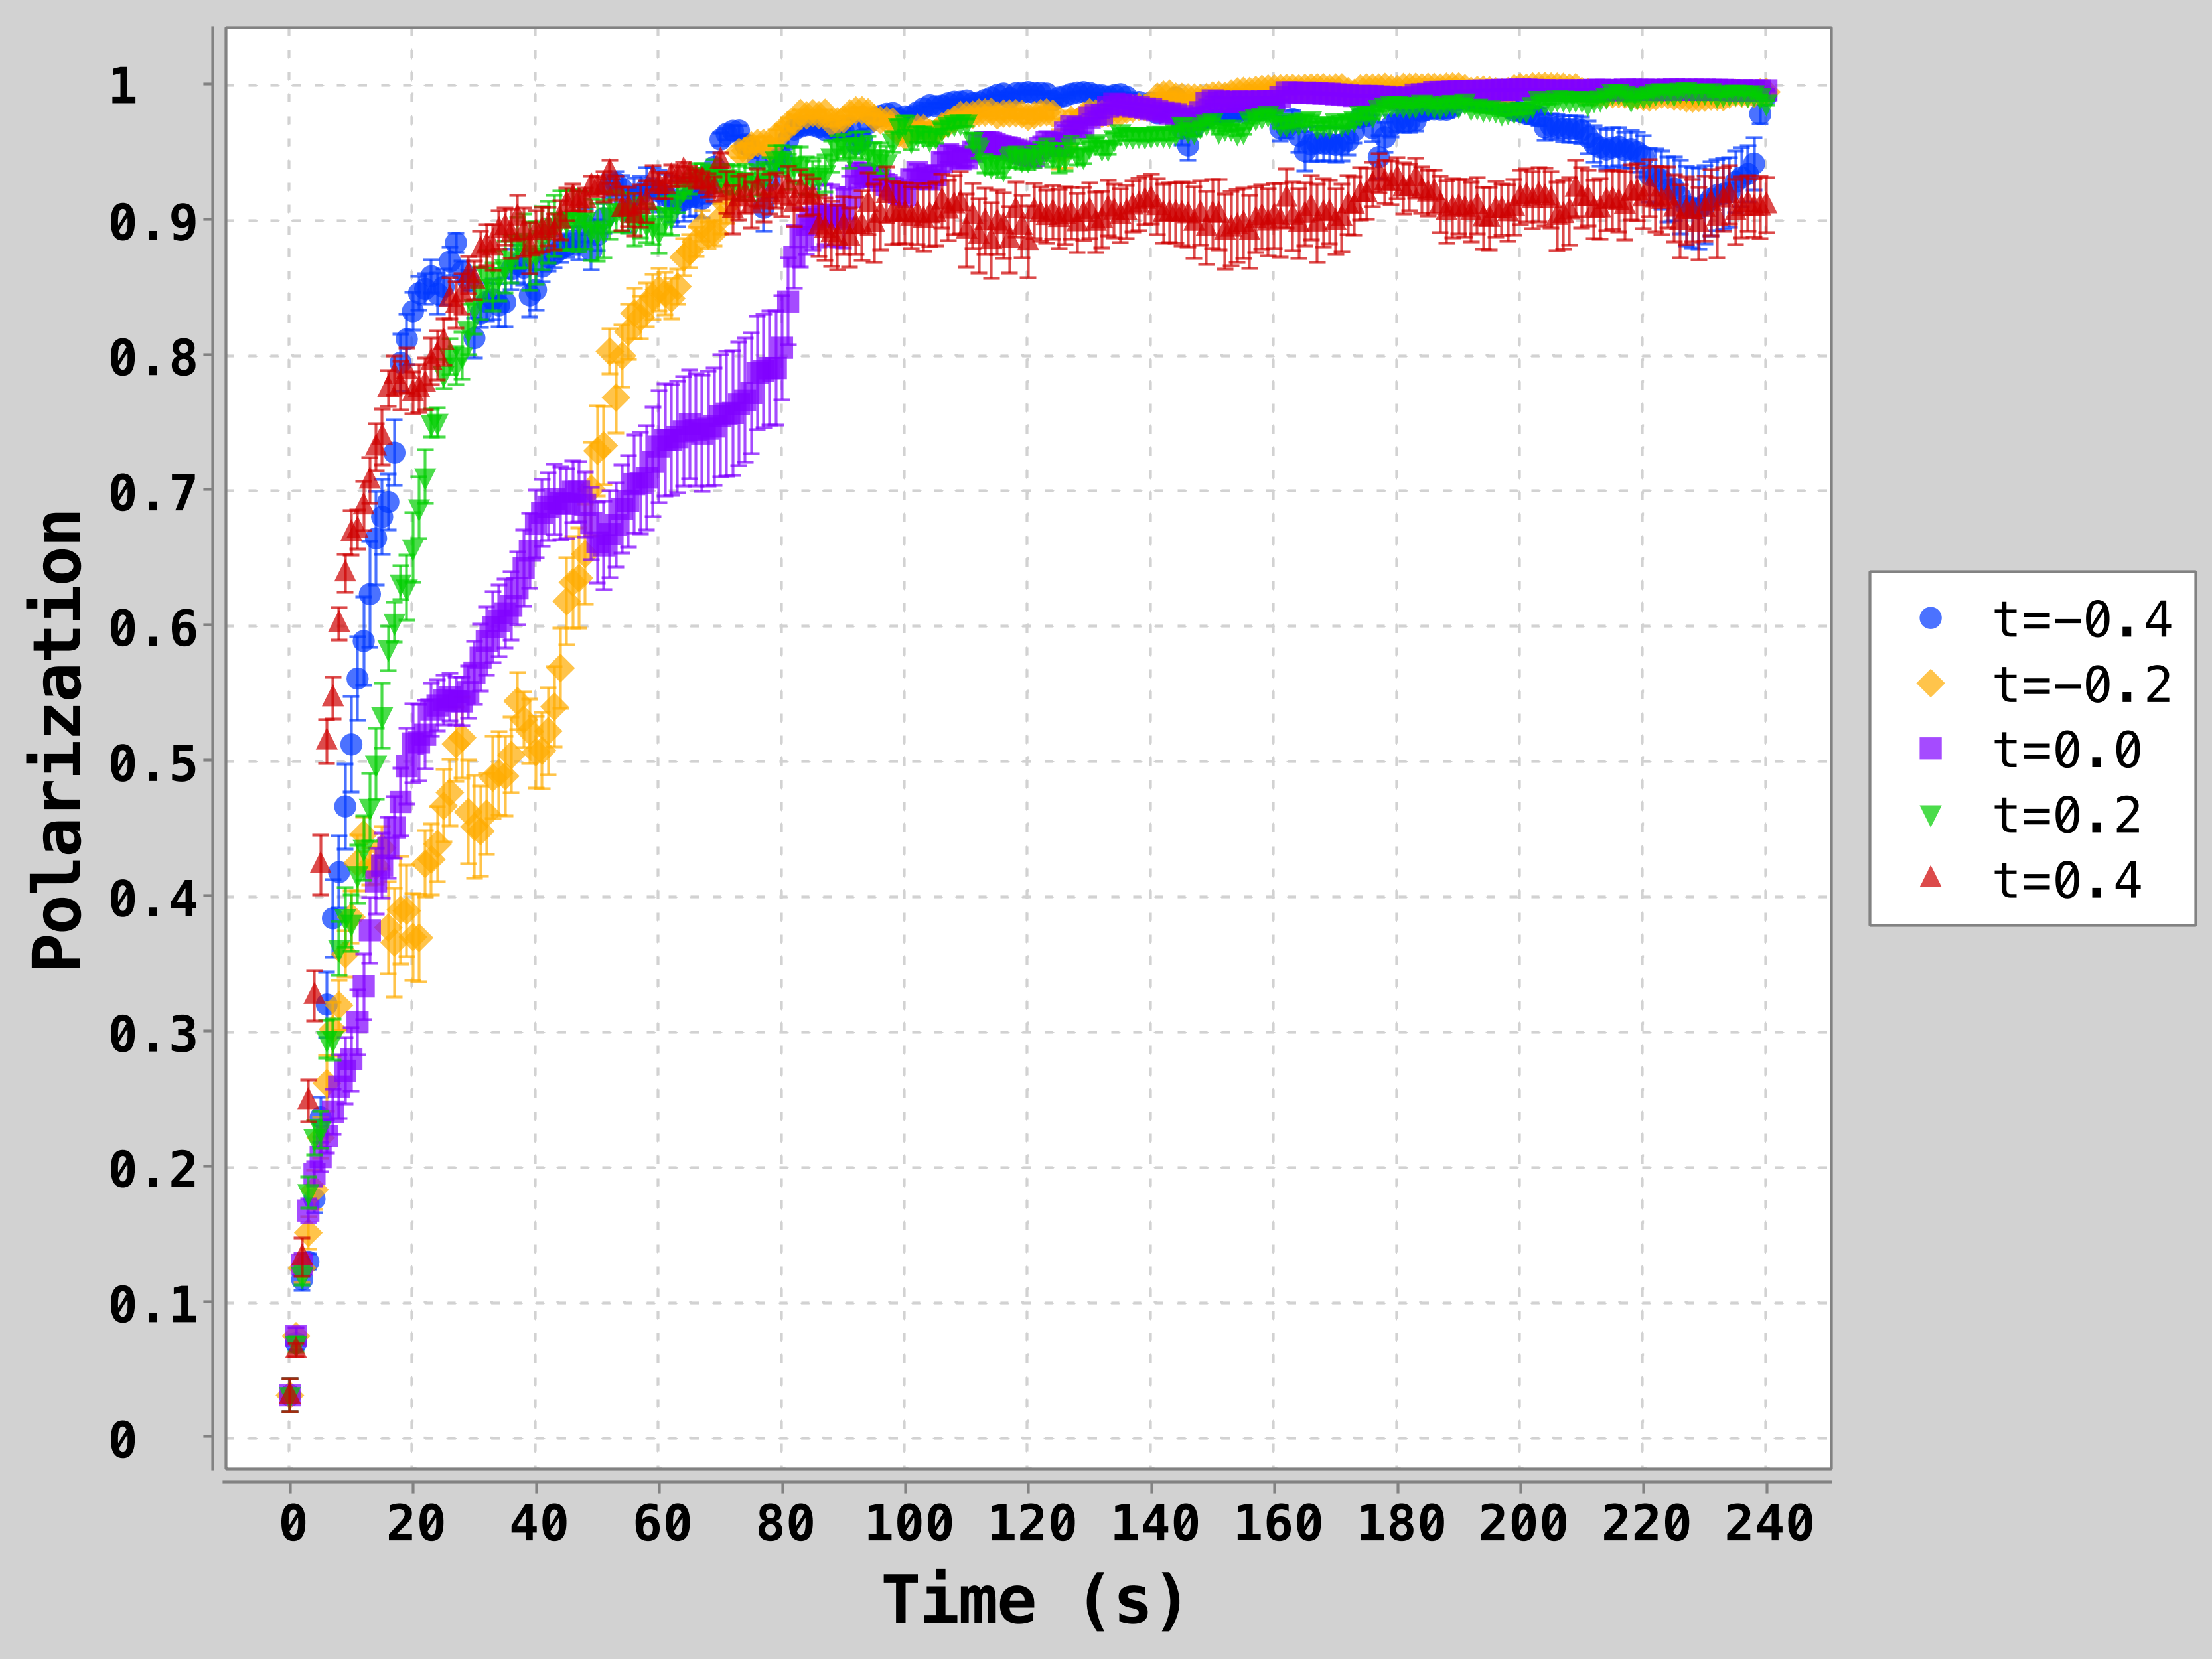
\includegraphics[width=\linewidth,height=\textheight,keepaspectratio]{{../imgs/polarization_t}.png}
        \end{frame}
        \begin{frame}
            \frametitle{1 - Polarización: Tendencia a}
            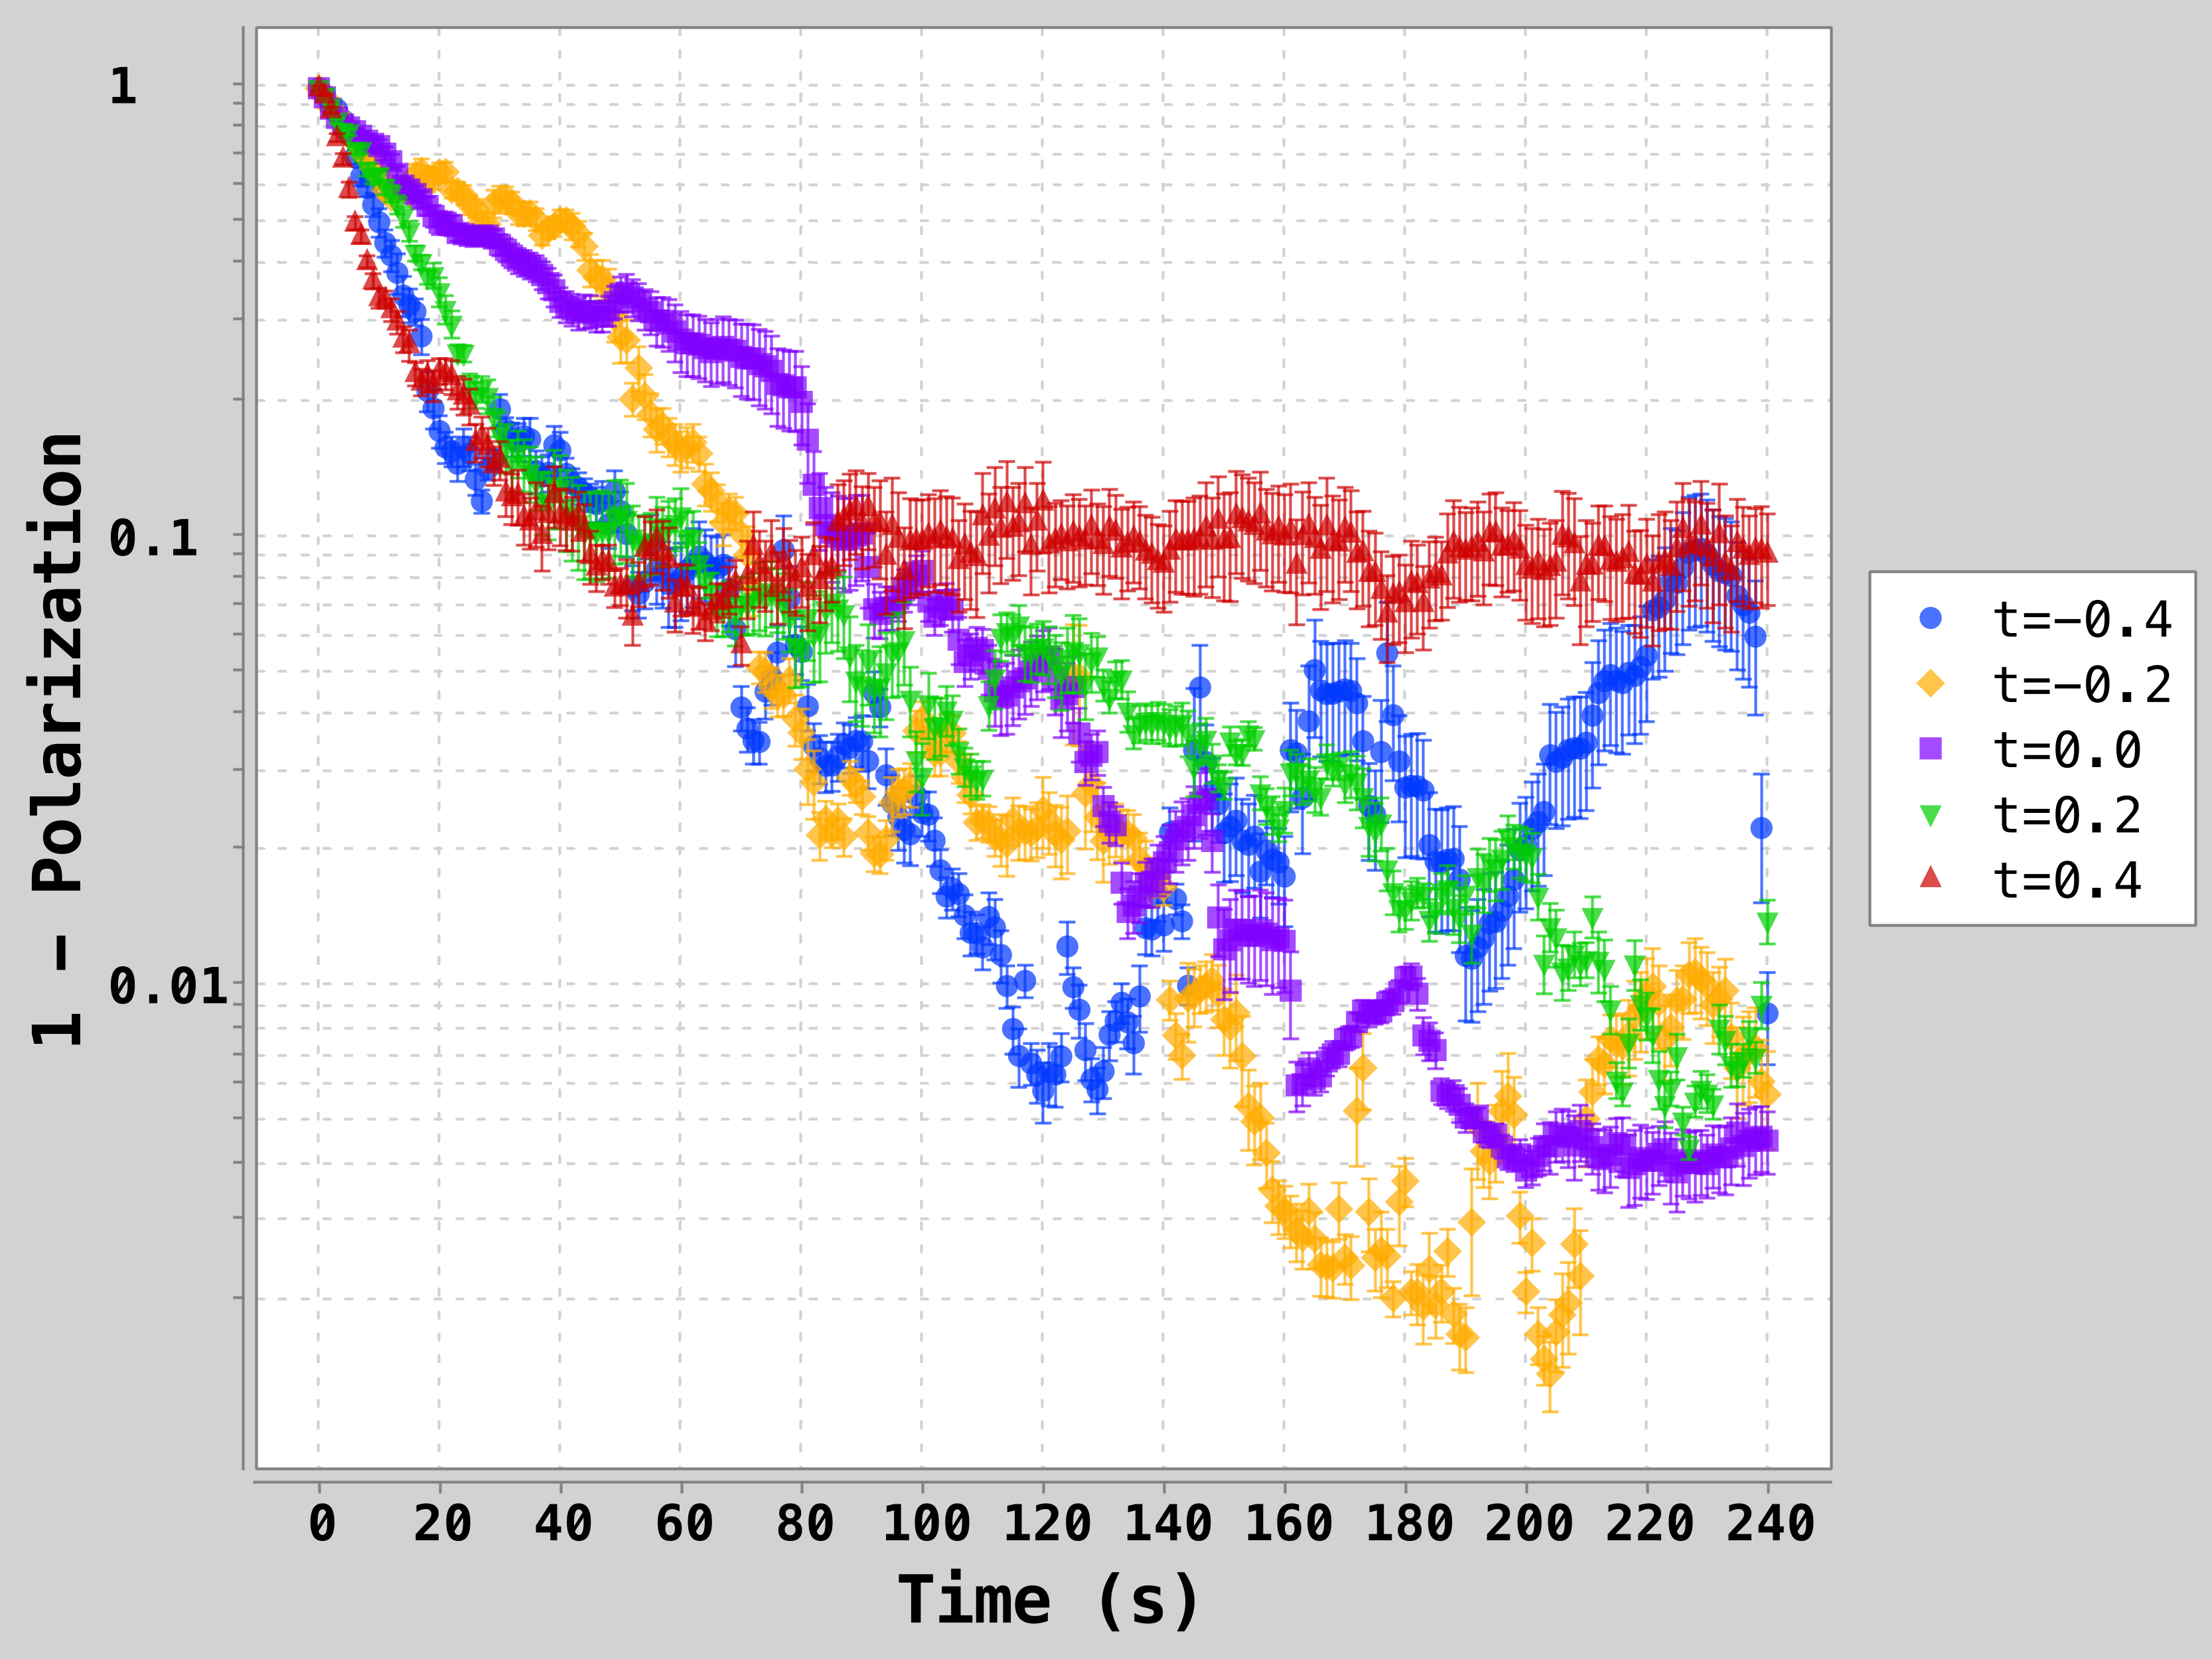
\includegraphics[width=\linewidth,height=\textheight,keepaspectratio]{{../imgs/polarization_t2}.png}
        \end{frame}
        \begin{frame}[standout]
            \frametitle{Tendencia a: t = 0.4 (2 boids especiales)}
            \begin{tikzpicture}[remember picture,overlay]
                \node[at=(current page.center)] {
                    \movie[width=0.55\paperwidth,height=0.55\paperwidth,showcontrols,autostart]
                    {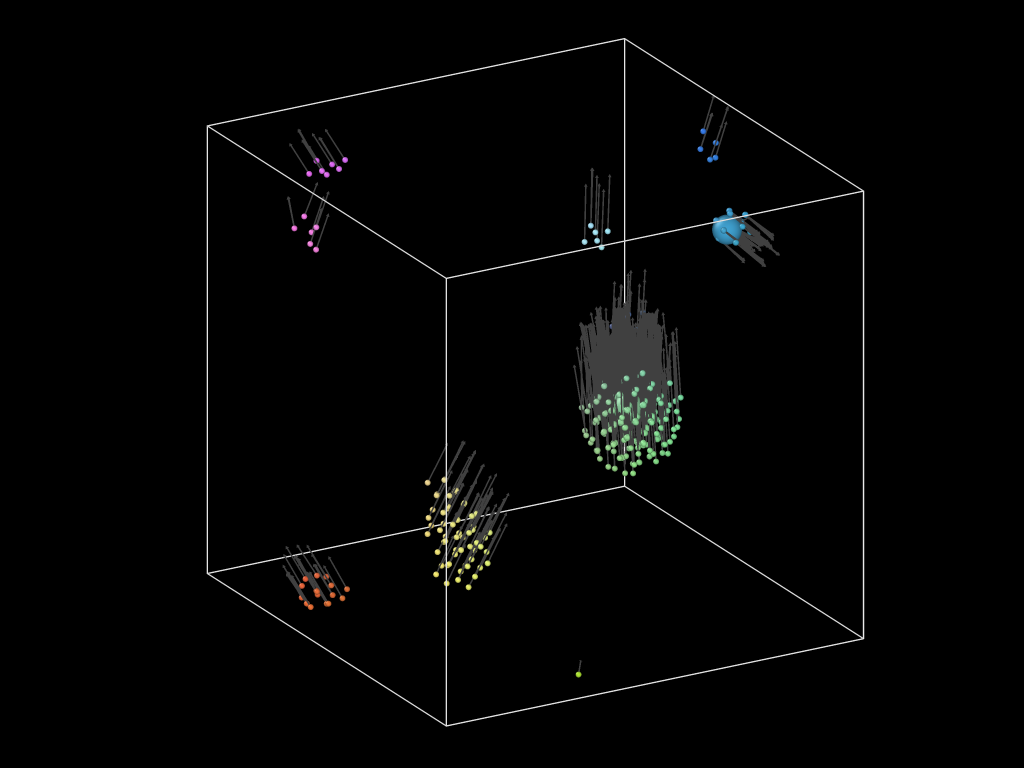
\includegraphics[width=0.55\paperwidth,height=0.55\paperwidth]
                        {../anims/universe__id_6456_t_0_4.png}
                    }
                    {../anims/universe__id_6456_t_0_4.mov}
                };
            \end{tikzpicture}
        \end{frame}

        \begin{frame}[standout]
            \frametitle{Tendencia a: t = -0.4 (2 boids especiales)}
            \begin{tikzpicture}[remember picture,overlay]
                \node[at=(current page.center)] {
                    \movie[width=0.55\paperwidth,height=0.55\paperwidth,showcontrols,autostart]
                    {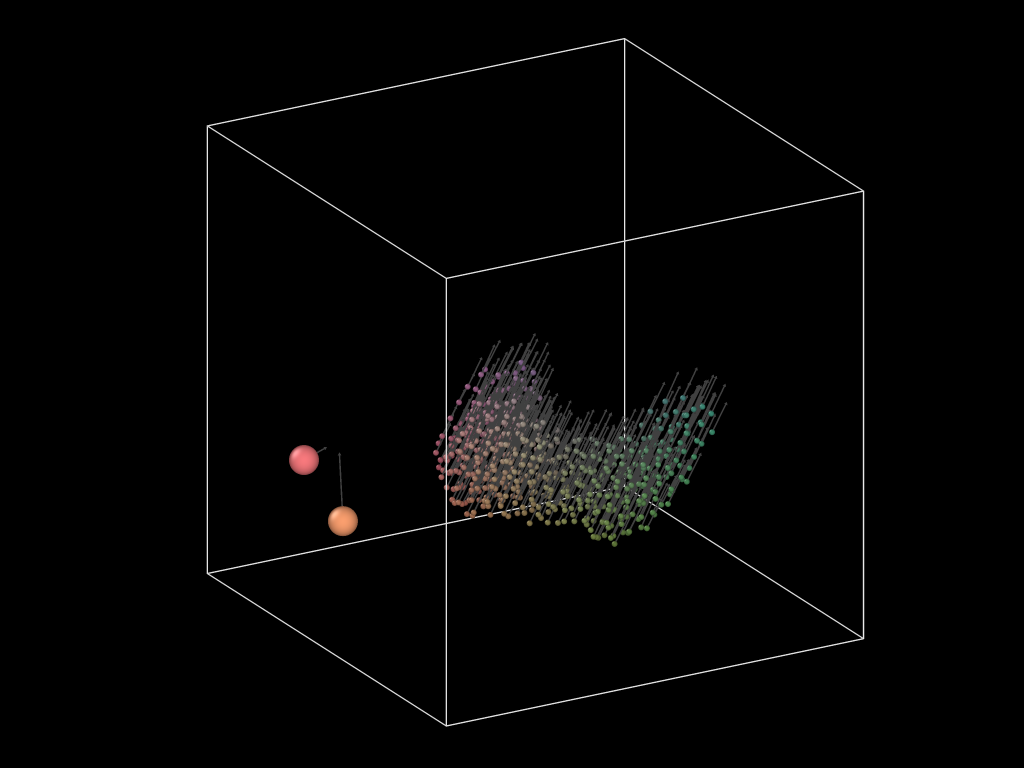
\includegraphics[width=0.55\paperwidth,height=0.55\paperwidth]
                        {../anims/universe__id_6456_t_-0_4.png}
                    }
                    {../anims/universe__id_6456_t_-0_4.mov}
                };
            \end{tikzpicture}
        \end{frame}
    \section{Conclusiones}
    \begin{frame}
        \frametitle{Conclusiones}
        \begin{itemize}
            \item La regla más importante para polarización: \textbf{Alineamiento}.
            \item Desactivar la regla de \textbf{Cohesión} acelera la polarización.
            \item Regla de \textbf{Tendencia a} cambia en gran medida el comportamiento de los \textit{boids}.
        \end{itemize}
    \end{frame}
    \end{document}
